\documentclass{tufte-book}

\hypersetup{colorlinks} % Comment this line if you don't wish to have colored links

\usepackage{microtype} % Improves character and word spacing

\usepackage{lipsum} % Inserts dummy text

\usepackage{booktabs} % Better horizontal rules in tables

\usepackage[type={CC}, modifier={by-sa}, version={4.0}]{doclicense}

\usepackage{graphicx} % Needed to insert images into the document
\graphicspath{{graphics/}} % Sets the default location of pictures
\setkeys{Gin}{width=\linewidth,totalheight=\textheight,keepaspectratio} % Improves figure scaling

\usepackage{textcomp} % gives a cent sign
\usepackage{ifsym} % \textifsym{0123456789} gives 7-segment display characters

\usepackage{tikz}
\usetikzlibrary{circuits.logic,circuits.logic.US,arrows,calc,automata,positioning}

\usepackage{tikz-timing}

% from http://tex.stackexchange.com/questions/47765/how-can-i-add-some-enhancement-to-the-matrix
\newcommand{\tikzmark}[1]{\tikz[overlay,remember picture] \node (#1) {};}
\newcommand{\DrawBox}[3][]{%
    \tikz[overlay,remember picture]{%
        \coordinate (TopLeft)     at ($(#2)+(-0.2em,0.9em)$);
        \coordinate (BottomRight) at ($(#3)+(0.2em,-0.3em)$);
        %
        \draw [black,thick,rounded corners,#1] (TopLeft) rectangle (BottomRight);
    }
}
\newcommand{\DrawBoxS}[3][]{%
    \tikz[overlay,remember picture]{%
        \coordinate (TopLeft)     at ($(#2)+(-0.2em,0.9em)$);
        \coordinate (BottomRight) at ($(#3)+(0.2em,-0.3em)$);
        \coordinate (BottomLeft)  at (TopLeft |- BottomRight);
        \coordinate (TopRight)    at (TopLeft -| BottomRight);
        %
        \draw [black,thick,rounded corners,#1] (BottomLeft) |- ($(TopLeft)!0.5!(TopRight)$) -| (BottomRight);
    }
}
\newcommand{\DrawBoxN}[3][]{%
    \tikz[overlay,remember picture]{%
        \coordinate (TopLeft)     at ($(#2)+(-0.2em,0.9em)$);
        \coordinate (BottomRight) at ($(#3)+(0.2em,-0.3em)$);
        \coordinate (BottomLeft)  at (TopLeft |- BottomRight);
        \coordinate (TopRight)    at (TopLeft -| BottomRight);
        %
        \draw [black,thick,rounded corners,#1] (TopLeft) |- ($(BottomLeft)!0.5!(BottomRight)$) -| (TopRight);
    }
}
\newcommand{\DrawBoxW}[3][]{%
    \tikz[overlay,remember picture]{%
        \coordinate (TopLeft)     at ($(#2)+(-0.2em,0.9em)$);
        \coordinate (BottomRight) at ($(#3)+(0.2em,-0.3em)$);
        \coordinate (BottomLeft)  at (TopLeft |- BottomRight);
        \coordinate (TopRight)    at (TopLeft -| BottomRight);
        %
        \draw [black,thick,rounded corners,#1] (TopLeft) -| ($(TopRight)!0.5!(BottomRight)$) |- (BottomLeft);
    }
}
\newcommand{\DrawBoxE}[3][]{%
    \tikz[overlay,remember picture]{%
        \coordinate (TopLeft)     at ($(#2)+(-0.2em,0.9em)$);
        \coordinate (BottomRight) at ($(#3)+(0.2em,-0.3em)$);
        \coordinate (BottomLeft)  at (TopLeft |- BottomRight);
        \coordinate (TopRight)    at (TopLeft -| BottomRight);
        %
        \draw [black,thick,rounded corners,#1] (TopRight) -| ($(TopLeft)!0.5!(BottomLeft)$) |- (BottomRight);
    }
}

\newcommand{\engAND}{\mathbin{\textsc{and}}}
\newcommand{\engOR}{\mathbin{\textsc{or}}}
\newcommand{\engXOR}{\mathbin{\textsc{xor}}}
\newcommand{\engNOT}{\mathop{\textsc{not}}}

\newcommand{\0}{\ensuremath{\mathtt{0}}}
\newcommand{\1}{\ensuremath{\mathtt{1}}}

% Get a better looking caret in tt-mode
%\usepackage{inconsolata}

% Use commands within \Verb and \Verbatim
\usepackage{fancyvrb}
\fvset{commandchars=\\\{\},commentchar=none}
\fvset{fontsize=\normalsize} % The font size of all verbatim text can be changed here

% Typeset #1 centered on the space that #2 would have occupied
\newcommand{\CenterSpace}[2]{\savebox{0}{#2}\savebox{2}{}\ht2=\ht0 \dp2=\dp0 \wd2=0.5\wd0
    \usebox{2}\makebox[0pt][c]{#1}\usebox{2}}

\newcommand{\Caret}{{\CenterSpace{\raisebox{-0.25ex}{\Large\textasciicircum}}{x}}}
\newcommand{\Tilde}{{\ \llap{\Large\textasciitilde}{}}}

\newenvironment{tailquote}{\par\begin{fullwidth}\hfill\begin{minipage}[t]{\textwidth}\raggedright\itshape}{\end{minipage}\end{fullwidth}}

\newcommand{\firstthought}[1]{\noindent\textsc{#1}}

\makeatletter 
\newcommand\mynobreakpar{\par\nobreak\@afterheading} 
\makeatother
\newenvironment{exercises}{\paragraph{Exercises}~\mynobreakpar\begin{enumerate}}{\end{enumerate}}

\setcounter{secnumdepth}{2} % numbered subsections

\newcommand{\hangp}[1]{\makebox[0pt][r]{(}#1\makebox[0pt][l]{)}} % New command to create parentheses around text in tables which take up no horizontal space - this improves column spacing
\newcommand{\hangstar}{\makebox[0pt][l]{*}} % New command to create asterisks in tables which take up no horizontal space - this improves column spacing

\usepackage{xspace} % Used for printing a trailing space better than using a tilde (~) using the \xspace command

\newcommand{\monthyear}{\ifcase\month\or January\or February\or March\or April\or May\or June\or July\or August\or September\or October\or November\or December\fi\space\number\year} % A command to print the current month and year

\newcommand{\openepigraph}[2]{ % This block sets up a command for printing an epigraph with 2 arguments - the quote and the author
\begin{fullwidth}
\sffamily\large
\begin{doublespace}
\noindent\allcaps{#1}\\ % The quote
\noindent\allcaps{#2} % The author
\end{doublespace}
\end{fullwidth}
}

\newcommand{\blankpage}{\newpage\hbox{}\thispagestyle{empty}\newpage} % Command to insert a blank page

\usepackage{makeidx} % Used to generate the index
\makeindex % Generate the index which is printed at the end of the document

\title[Foundations of Computation]{%
  \setlength{\parindent}{0pt}Foundations\\ of\\ Computation}
\author{Brian T. Howard}
\publisher{Castle Howard Publishing}

\begin{document}
\setcounter{tocdepth}{2}
\frontmatter

%\thispagestyle{empty}
%\openepigraph{Quotation 1}{Author, {\itshape Source}}
%\vfill
%\openepigraph{Quotation 2}{Author}
%\vfill
%\openepigraph{Quotation 3}{Author}

\maketitle

\newpage
\begin{fullwidth}
~\vfill
\thispagestyle{empty}
\setlength{\parindent}{0pt}
\setlength{\parskip}{\baselineskip}
Copyright \copyright\ \the\year\ \thanklessauthor

\par\smallcaps{Published by \thanklesspublisher}

\par\url{http://www.csc.depauw.edu/~bhoward/}

\par \doclicenseThis\index{license}

\par\textit{First printing, \monthyear}
\end{fullwidth}

\tableofcontents

\listoffigures

\listoftables

\cleardoublepage
~\vfill
\begin{doublespace}
\noindent\fontsize{18}{22}\selectfont\itshape
\nohyphenation
Dedicated to Eleanor\index{Howard, Eleanor},\\
George\index{Howard, George}, Susanna\index{Howard, Susanna}, and Alice\index{Howard, Alice}.
\end{doublespace}
\vfill
\vfill

\cleardoublepage
% !TEX root = ../root.tex

\chapter{Introduction}
\firstthought{Computation is an inherently mathematical activity.} This is not to say that computation is all about adding and multiplying numbers, any more than mathematics is all about arithmetic. Indeed, just as practicing mathematicians can spend an entire career without needing to perform long division or solve a quadratic equation, many computer scientists and software developers will rarely perform tasks that resemble the math taught in school.

In 1995, the text \textit{Foundations of Computer Science}, by Alfred V. Aho\index{Aho, Alfred V.} and Jeffrey D. Ullman\index{Ullman, Jeffrey D.}\cite{aho1994foundations}, provided an excellent introduction to a broad range of topics at the mathematical core of computer science. However, in the intervening two decades, much has changed in the field, from the shifting fashions of popular programming languages to the rise of the World Wide Web. Although the core topics remain largely unchanged, the motivating examples and the means by which they are presented need to be revised to accommodate the new generation of students and current challenges in the computing profession.

The goal of this text is to adapt the classic Aho \& Ullman work to provide a better fit to the current curriculum of several of DePauw's Computer Science courses. In addition to CSC 233, Foundations of Computation, which has used sections of Aho \& Ullman for the past several years, portions of the book are also relevant to the companion sophomore-level courses (CSC 231, Computer Systems and CSC 232, Object-Oriented Software Development), as well as several of the upper-level courses.

One significant advantage of ensuring that students come into the upper-level courses with a more substantial mathematical background is that many of the common tools of computer science may be moved into the common core instead of being introduced and re-introduced in multiple later courses. Examples of these common tools include the interconnected notions of
\begin{itemize}
\item tree-like hierarchical data,
\item systems of grammar rules,
\item patterns of function evaluation, and
\item simple digital logic circuits,
\end{itemize}
or their corresponding generalizations to
\begin{itemize}
\item web-like networked data,
\item systems of states and transition rules,
\item patterns of recursive functions, and
\item logic circuits with feedback and memory.
\end{itemize}

The disadvantage of the Aho \& Ullman text is that, although the core material will continue to be relevant for many years, the presentation has become dated in several ways. First, though not most important, is the programming language used for the book's examples. The original edition, in 1992, used Pascal, which by that time was already waning in popularity for teaching. The 1994 edition updated the examples to C, which has shown considerably more staying power, either in its plain form or in the updated C++. However, that edition just missed the boat on the most popular programming language of the past 20 years, Java, which was introduced to the public the following year.

That year also saw an explosion of interest in the World Wide Web, fueled in part by Java's ability to add interactivity to webpages that initially had only contained static text and images. This was the start of the more serious relevance problems for \textit{Foundations of Computer Science}: it has no mention of the single most influential application of networked data, the web. Other foundational computer science topics that have since risen in importance, but which are at most only hinted at by Aho \& Ullman, include: parallel computing (which has become essential in recent years with the spread of multicore processors), distributed computing (such as the massive server farms at Google, or the notion of ``computing in the cloud''), security (encryption techniques rely heavily on mathematics), and additional programming paradigms such as object-oriented, logic, and functional programming.

This last point, the use of functional programming, is particularly important to our presentation of CSC 233. The functional style\index{functional style} has close ties with the mathematical roots of our subject, and fits well with topics such as handling hierarchical data and working with recursion. The absence of functional programming from Aho \& Ullman is certainly the most glaring mismatch between the text and the course.

Finally, one of the other core topics that migrated into DePauw's Foundations course is digital logic. This used to be a part of Computer Systems, but it is currently included in Foundations because it fits well with the other topics, and it makes room in Systems for additional higher-level material. Aho \& Ullman have a chapter on digital logic, but it is not as comprehensive; uncharacteristically, they only hint at the generalization from straight-line, tree-like combinational circuits to sequential circuits with feedback loops. This is particularly unfortunate, because this topic makes a good course wrap-up, tying together several previous threads (namely, it applies the graph data model and finite state transition diagrams to turn the pure functional logic circuits into machines with memory).


\mainmatter

% !TEX root = ../root.tex

% !TEX root = ../root.tex

\chapter{Functional Programming}
% !TEX root = ../root.tex

\section{Introduction to Scala}
\firstthought{The Scala programming language} is a relative of Java that enables what is known as a ``functional'' programming style; what this means will be the subject of much of the rest of this chapter. This introduction assumes that you are already familiar with programming in Java and/or C++. You may not be an expert, but you are comfortable with writing classes and methods. We will by no means be learning all of Scala here, and when there are multiple ways to express something in Scala we will generally just choose one. The emphasis is on becoming able to read and write simple functions to manipulate the kinds of data models talked about in the Foundations class: lists, trees, graphs, \textit{etc}. Although Scala also has extensive support for an object-oriented style of programming, we will be focusing on its support for functional programming.

Before diving into the details, here is a short sales pitch for Scala. This is a quote from the main Scala website, \url{http://www.scala-lang.org/}:
\begin{quotation}
Scala\index{Scala} is a general purpose programming language designed to express common programming patterns in a concise, elegant, and type-safe way. Scala smoothly integrates features of object-oriented and functional languages, enabling developers to be more productive while retaining full interoperability with Java and taking advantage of modern multicore hardware.
\end{quotation}
Scala is a real-world, commercial-strength language, being used at companies such as Twitter, LinkedIn, Verizon, and many others; one of its attractions to these businesses is that it is very compatible with existing Java code, while also supporting more advanced programming techniques as found in functional languages such as Haskell and F$^\sharp$, or in dynamic languages such as Python and Ruby.

The ``functional'' programming style referred to above is not meant to imply that other styles are dysfunctional; rather, it refers to an emphasis on building programs out of pure functions. A pure function\index{pure function}\index{function!pure} is a block of code whose result depends only on the values of its input parameters; just like a function in mathematics, every time it is called with the same arguments it will return the same result. Furthermore, calling a pure function must have no side-effects\index{side-effect}---it will not change the state of any external variable, nor perform input or output, nor throw an exception.

Clearly we do not want to write entire programs with no side-effects, since they could never interact with the user. However, the functional style\index{functional style} encourages a program structure where all external effects are handled at the outermost layer, with the main body of the program composed entirely out of pure functions. There are many advantages to this design: functional code is easier to reason about and to test, it is more likely to be reusable, and it may well be easier to optimize for different hardware configurations, such as multicore processors or distributed clusters.

One consequence of performing a computation in a pure function is that it has a property known as ``referential transparency.''\index{referential transparency} The essence of this is that a function call may be replaced by its result value at any point in a program without affecting the behavior of the program (except perhaps its running time). This enables us to reason about functional programs using a substitution model,\index{substitution model} just as used in algebra: if we know that the referentially transparent expressions $e_1$ and $e_2$ are equal, then whenever we see $e_1$ in a program we may replace it with $e_2$.

Here is an example of a Java function that is \emph{not} pure:\index{function!impure}
\begin{verbatim}
public int double(int n) {
  System.out.println("Doubling " + n);
  runningTotal += n;
  return 2 * n;
}
\end{verbatim}
Each time \verb|double(n)| is called, it has two side-effects:\index{side-effect} it prints a message to the console and it modifies an external variable (\verb|runningTotal|, which is presumably an instance variable or static field of a containing class). Now consider the following program fragment:
\begin{verbatim}
int x = double(3) * double(3)
\end{verbatim}
The resulting value of \verb|x| will be 36, but the net effect of executing that statement in Java will be different from either of the following:
\begin{verbatim}
int y = double(3);
int x = y * y;
\end{verbatim}
or
\begin{verbatim}
int x = 6 * 6;
\end{verbatim}
When we deal with impure functions, our ability to reason about and manipulate code becomes significantly more complicated than just performing substitution.

In Scala, a pure function definition will have the following form:\index{Scala!function definition}
\begin{verbatim}
def <function-name>(<parameters>): <type> = <expression>
\end{verbatim}
The parameters\index{Scala!parameters} should be a comma-separated list of zero or more entries of the form \verb|<variable-name>: <type>|. Variable and function names\index{Scala!identifiers} follow the usual rules for Java identifiers (with some extensions we will see later): they must start with a letter, and consist of letters, digits, or underscores. The expression on the right-hand side should have the given return type;\index{Scala!return type}\footnote{In many cases Scala can infer\index{type inference} the return type if it is not provided, but we will see an important case where it cannot, so it is a good habit to always specify it.} it may be a simple expression or a block surrounded by braces.\index{Scala!block} If it is a block, then all but the last statement should be definitions of local functions or constants;\footnote{We will see later that blocks may also contain local import statements and definitions of objects, classes, traits, or types. Statements before the end of the block can also be expressions, but since they could only be evaluated for their side-effects,\index{side-effect} we will not need this in functional code.} the last statement will be the expression whose value is returned. A constant definition\index{Scala!constant definition} has the form:
\begin{verbatim}
val <variable-name> = <expression>
\end{verbatim}
An explicit type may be given after the name, such as \verb|val n: Int = 42|, but Scala is usually able to infer the correct type without this.

For example, here is a function that returns the square of the double of its integer argument (there are simpler ways to do this, but we want to explore the possibilities):
\begin{verbatim}
def squareDouble(k: Int): Int = {
  def double(n: Int): Int = 2 * n
  val x = double(k)
  x * x
}
\end{verbatim}
Note that, in addition to the placement of the type annotation \emph{after} the variable, Scala has another minor syntactic difference from Java: semicolons are optional at the end of a line.

As an example of reasoning by substitution,\index{substitution model} here is one way to evaluate a function call such as \verb|squareDouble(3)|:
\[ \begin{array}{rcl}
\verb|squareDouble(3)| & = & \verb|x * x|,\quad
\begin{array}[t]{l}
\textit{where }\verb|x = double(3)|\\
\textit{and }\verb|double(n) = 2 * n|
\end{array}\\
& = & \verb|x * x|,\quad
\begin{array}[t]{l}
\textit{where }\verb|x = 2 * 3|
\end{array}\\
& = & \verb|x * x|,\quad
\begin{array}[t]{l}
\textit{where }\verb|x = 6|
\end{array}\\
& = & \verb|6 * 6|\\
& = & \verb|36|
\end{array} \]

We will occasionally have need of modifiable local variables,\index{Scala!variable definition} which are defined like constants but use the keyword \verb|var| instead of \verb|val|. A variable may be assigned\index{Scala!assignment} a new value after definition with an assignment statement, just as in Java:
\begin{verbatim}
var x = 1
x = x + 1  // after this, x will be 2
\end{verbatim}
However, this reduces the purity of the code (reasoning about an expression containing \verb|x| needs to take into account what its current value is, whether it is before or after an assignment), and in general we will prefer ``immutable''\index{immutability} variables (\textit{i.e.}, constants). When we deal with larger data structures, this preference for immutability will continue.

\begin{tailquote}
In 1977, John Backus\index{Backus, John} (1924--2007)---one of the inventors of the Fortran programming language---was awarded the highest prize in computing, the Turing Award. The lecture he gave at the award ceremony was titled ``Can Programming Be Liberated from the von Neumann Style? A Functional Style and Its Algebra of Programs.'' Backus enumerated many of the problems he had seen with languages such as Fortran, and his algebraic approach to reasoning about pure expression-based programs influenced much subsequent research in functional programming.
\end{tailquote}
\begin{exercises}
\item Consider the following Scala function:
\begin{verbatim}
def exercise(a: Int, b: Int): Int = {
  def m(x: Int, y: Int): Int = x - y
  def s(n: Int): Int = n * n
  val c = m(a, b)
  val d = m(a, c)
  val e = c + d
  s(d) - s(e)
}
\end{verbatim}
\begin{enumerate}
\item What is the value of \verb|exercise(4, 5)|?
\item What is the value of \verb|exercise(12, 13)|?
\item Use algebraic substitution to evaluate \verb|exercise(a, b)| in terms of the variables \verb|a| and \verb|b|.
\end{enumerate}

\item Write a Scala function named \verb|average| that takes three integer arguments and calculates their average. For example, \verb|average(7, 1, 2)| should return \verb|3| (use integer division, which rounds toward zero).

\item Write a Scala function named \verb|median| that takes three integer arguments and calculates their median (that is, the middle of the three numbers when they are put in increasing order). For example, \verb|median(7, 1, 2)| should return \verb|2|. You may use the library functions \verb|math.min(a, b)| and \verb|math.max(a, b)|, which respectively return the smaller and the larger of their arguments.
\end{exercises}

\section{Types}
\firstthought{While it is not strictly necessary} to have explicit types\index{types} for a language to be functional, it is important to have a notion (perhaps only in the programmer's mind) of the range of values allowed for a given variable or expression, as well as the ways it may be used (for example, whether it may be applied to an argument). Scala has a rich set of mechanisms for describing types, and the compiler will check that the explicitly declared types in a program are consistent.

In this and following sections, we will walk through a useful subset of these types, and describe the corresponding code constructs for operating on them. One recurrent theme will be that the type of the data determines the structure of the program; once you know the input and output types of a function, you can often lay out a skeleton for how the function must be written.

\paragraph{Booleans}
\firstthought{The simplest type} conveying a non-trivial amount of information is the common \verb|Boolean| type,\index{types!Boolean} whose values may only be \verb|true| or \verb|false|. Scala has the usual relational operators\index{Scala!relational operators}\index{operators!relational} (\verb|==|, \verb|!=|, \verb|<=|, \textit{etc}.) familiar from Java and other C-derived languages; the only difference here is that the equality test defaults to checking equality of values, rather than just object identity (so you do not have to remember to use \verb|.equals| on strings\ldots). It also has the familiar logical operators\index{Scala!logical operators}\index{operators!logical} \verb|&&| (\textsc{and}), \verb-||- (\textsc{or}), and \verb|!| (\textsc{not}).

The obvious way to use a Boolean value is with an \verb|if| expression\index{Scala!if expression}:
\begin{verbatim}
if (<test>) <true-clause> else <false-clause>
\end{verbatim}
If the expression \verb|<test>| evaluates to \verb|true|, then the whole expression evaluates to \verb|<true-clause>|, otherwise it evaluates to \verb|<false-clause>|. Note that, in Scala, \verb|if| is an \emph{expression} rather than a statement---it may be used anywhere a value is needed that depends on the result of a test. For example, here is an absolute value function:
\begin{verbatim}
def absoluteValue(x: Double): Double = if (x >= 0) x else -x
\end{verbatim}

Another running theme in Scala is the use of ``pattern matching''\index{Scala!match expression}\index{pattern matching} to take values apart. For a Boolean value, the appropriate pattern match takes the following form:
\begin{verbatim}
<test> match {
  case true => <true-clause>
  case false => <false-clause>
}
\end{verbatim}
The behavior in this case is exactly the same as the above \verb|if| expression; performing this operation on Booleans is so common that the shorter \verb|if| form is generally used.

\paragraph{Primitives}
\firstthought{Scala is usually compiled} to run on the same virtual machine as Java (although there are other alternatives), so it is not surprising that it offers the same range of primitive types\index{types!primitive} as Java. Just about the only difference is that the type names are capitalized: integers are \verb|Int|, floating-point numbers are \verb|Double|, and characters are \verb|Char|. We will stick to these primitive types in this book, although the others (such as \verb|Long|, \verb|Byte|, and \verb|Float|) are also available.\footnote{The intuition for primitive values is that they can be stored in a small, fixed number of bytes and operated on by single machine instructions.}

All of the usual literal constants\index{Scala!literals} and operators are carried over from Java, except the ``cast'' operation is not directly supported. If you want to convert a \verb|Double| to an \verb|Int|, for example, use the \verb|toInt| method:\footnote{Note that, unlike Java, Scala treats even primitive values as if they were objects with methods.} \verb|x.toInt| instead of \verb|(int) x|.

One interesting generalization in Scala is that all operators\index{Scala!operators}\index{operators!Scala} are treated as method calls. For example, \verb|a + b| is compiled as if it were \verb|a.+(b)|. This allows us to extend the available operators by defining our own methods with ``symbolic'' names. In fact, operators don't need to be symbols---any single-argument method may be used as an operator. Thus, the \verb|max| method on numbers, where \verb|a.max(b)| is the larger of \verb|a| and \verb|b|, may also be written as \verb|a max b|.

Pattern matching\index{pattern matching} on primitives looks like the usual \verb|switch|/\verb|case| statement from C and Java, except as above it produces an expression whose value is given by the matching case:
\begin{verbatim}
def factorial(n: Int): Int = n match {
  case 0 => 1
  case _ => n * factorial(n - 1)
}
\end{verbatim}
The second case in this example uses the ``wildcard'' pattern,\index{wildcard}\index{_@\_} \verb|_| (underscore). This pattern matches anything, so it serves as the \emph{default} case. This example also demonstrates defining a function recursively,\index{function!recursive} where the value at one argument depends on first computing the value for some other argument; we will have much more to say about this below.\footnote{Defining a recursive function is the situation mentioned above where the compiler is not always able to infer a return type;\index{Scala!return type}\index{type inference} in the example, it would have to know that \texttt{factorial} returns an \texttt{Int} before it could figure out the type on the right-hand side.}

Patterns may also have ``guard''\index{Scala!guard expression} expressions---tests that have to evaluate to \verb|true| for the case to match. For example, here is a match that converts a character representing a hexadecimal digit to its integer value; if the digit is invalid, it returns \verb|-1|:
\begin{verbatim}
digit match {
  case d if '0' <= d && d <= '9' => d - '0'
  case d if 'A' <= d && d <= 'F' => d - 'A' + 10
  case d if 'a' <= d && d <= 'f' => d - 'a' + 10
  case _ => -1
}
\end{verbatim}

\paragraph{Strings}
\firstthought{A Scala string}\index{types!string}\index{Scala!strings} is literally the same as a Java string, at least when compiled to the Java VM. Some additional methods have been added for convenience, such as:
\begin{itemize}
\item \verb|head|, which returns the first character (\verb|s.head| is the same as \verb|s.charAt(0)|),
\item \verb|tail|, which returns all but the first character (\verb|s.tail| is the same as \verb|s.substring(1, s.length())|), and
\item \verb|toInt|, which attempts to parse an integer value from its string representation (\verb|s.toInt| is the same as \verb|Integer.parseInt(s)|).
\end{itemize}
Note that these methods, which are defined in terms of some underlying Java methods, are not strictly pure\index{function!impure}---in each case, they may throw an exception if the string doesn't satisfy some precondition (for \verb|head| and \verb|tail|, it must be non-empty; for \verb|toInt|, it must consist only of one or more digits, optionally preceded by a sign \verb|+| or \verb|-|). However, Java strings (unlike strings in C or C++) \emph{are} immutable, so at least no operation on a string can change the underlying character sequence.\index{immutability}

As mentioned above, strings may be compared for equality with the \verb|==| operator. They have also been extended with comparison operators,\index{Scala!relational operators}\index{operators!relational} so \verb|s < t| is true when \verb|s| lexically precedes \verb|t|.

A convenient extension in Scala is the ability to specify strings that contain special characters, such as quotes and newlines, by enclosing them in triple quotes (these are called ``raw strings''):\index{Scala!raw strings}
\begin{verbatim}
"""This is a string with several lines.
This is the second line, which contains a quotation: "Hello World".
This is the third line."""
\end{verbatim}
To make this easier when code is indented, there is a method named \verb|stripMargin| that will remove leading characters up to the first vertical bar on each line:
\begin{verbatim}
"""This is a string with several lines.
  |This is the second line, which contains a quotation: "Hello World".
  |This is the third line.""".stripMargin
\end{verbatim}

Another extension to the notation for strings is ``string interpolation.''\index{Scala!string interpolation}\index{$@\$} This is actually a very general and extensible facility in the language, but in its simplest form, if you prefix a string literal with the letter \verb|s|, then any occurrence of \verb|$|$x$ in the string will be replaced by the value of variable $x$ (converted to a string, if necessary). Instead of a single variable, an entire expression \textit{expr} may be interpolated if it is enclosed in braces: \verb|${|\textit{expr}\verb|}|. Here is an example:
\begin{verbatim}
s"The value of x is $x, and x*7 is ${x*7}."
\end{verbatim}
If $x$ is 6, then this evaluates to \verb|"The value of x is 6, and x*7 is 42."|

Pattern matching on strings is similar to that on primitives: each case specifies a string literal to be matched, or a guard expression to be satisfied.\index{pattern matching} Later in the book, when we see regular expressions, there will be a more general notion of pattern matching for strings.

\paragraph{Tuples}
\firstthought{If a function} needs to return more than one value, it is convenient to be able to package up several values into a single object. In Java, you might create a new class with the desired fields (think of the \verb|Point| class, with \verb|x| and \verb|y| fields). In Scala, a simpler option is to create a ``tuple''\index{types!tuple} (sometimes called an $n$-tuple,\index{n-tuple@$n$-tuple} where $n$ is the number of values). A tuple value is written by giving a comma-separated list of values in parentheses; for example, \verb|(42, "Hello World", false)|. The corresponding type is written as a list of types in parentheses; for example, \verb|(Int, String, Boolean)|.

A 2-tuple is also known as a pair\index{pair} (and a 3-tuple is a triple, \textit{etc.}). An interesting special case is the 0-tuple: the only value is the empty tuple, \verb|()|. The type of the empty tuple is \verb|Unit|;\index{types!unit} it plays the same role as \verb|void| in Java. A function that takes a \verb|Unit| argument might as well not take an argument, because the single value provides no information. A function that \emph{returns} the \verb|Unit| type is suspicious: if it doesn't return a value, then the only reason to call it must be to perform some side-effect.\index{side-effect} Indeed, one of the places we will encounter the \verb|Unit| type is as the return value of non-pure functions\index{function!impure} such as \verb|println|.

Individual elements of a tuple may be accessed with the methods \verb|_1|,\index{_1@\texttt{\_1}} \verb|_2|,\index{_1@\texttt{\_2}} \textit{etc.} However, it is often more natural to extract elements of a tuple with pattern matching.\index{pattern matching} For example, the \verb|splitAt| method on strings returns a pair of strings: \verb|s.splitAt(n)| yields \verb|(a, b)|, where \verb|a.length == n| and \verb|a + b == s|. We may extract these two strings from the pair\index{pair} as follows:
\begin{verbatim}
s.splitAt(n) match {
  case (first, second) =>
    s"""The first $n characters are "$first",
       |and the rest are "$second".""".stripMargin
}
\end{verbatim}
If \verb|s| is \verb|"Hello World"| and \verb|n| is 5, then the result of this expression is
\begin{verbatim}
The first 5 characters are "Hello",
and the rest are " World".
\end{verbatim}

Patterns may be combined, such as a tuple pattern containing literal or wildcard patterns. For example, here is one way to define a Boolean \textsc{and} function:
\begin{verbatim}
def and(x: Boolean, y: Boolean): Boolean = (x, y) match {
  case (false, _) => false
  case (_, false) => false
  case _ => true
}
\end{verbatim}
These cases say that if either \verb|x| or \verb|y| is \verb|false|, then the result is \verb|false|; otherwise it is \verb|true|. Note that the first two cases overlap: if \verb|x| and \verb|y| are both false, then both patterns will match. Scala always chooses the first case with a matching pattern (so a default case, if present, must occur last). Also notice the technique of combining \verb|x| and \verb|y| into a tuple so that the pattern match can depend on both.\index{pattern matching}

\begin{tailquote}
In programming, a type system serves to prevent certain kinds of errors when a program is run. Types\index{types} were used in the early 20\textsuperscript{th} century for a similar purpose: they prevented certain paradoxes when formalizing mathematical logic. This is not entirely coincidental---many aspects of computer hardware and programming languages were influenced by the work of logicians such as Alan Turing,\index{Turing, Alan} Alonzo Church,\index{Church, Alonzo} and Haskell Curry.\index{Curry, Haskell}
\end{tailquote}
\begin{exercises}
\item Consider this Scala function:
\begin{verbatim}
def foo(m: Int, n: Int): Int = n match {
  case 0 => 1
  case _ if n % 2 == 1 => m * foo(m, n - 1)
  case _ =>
    val p = foo(m, n / 2)
    p * p
}
\end{verbatim}
Recall that \verb|%| is the mod operator: \verb|a % b| is the remainder when \verb|a| is divided by \verb|b|.\index
\begin{enumerate}
\item What is the value of \verb|foo(3, 0)|?
\item What is the value of \verb|foo(3, 1)|?
\item What is the value of \verb|foo(3, 2)|?
\item What is the value of \verb|foo(3, 3)|?
\item What is the value of \verb|foo(3, n)|, in terms of \verb|n|?
\end{enumerate}

\item Write Scala functions that compute the inclusive and exclusive \textsc{or} operations. That is, write Boolean functions \verb|or(x, y)| and \verb|xor(x, y)| that will return \verb|true| if one of \verb|x| or \verb|y| is \verb|true|; in the inclusive case, \verb|or(true, true)| is also \verb|true|, while for the exclusive case, \verb|xor(true, true)| is \verb|false|. Use pattern matching for one, and \verb|if| expressions for the other (but do not use the built-in logical operators such as \verb-||-).

\item Define a function \verb|minmax(a: Int, b: Int)| that returns a pair of numbers, where the first is the smaller of \texttt{a} and \texttt{b}, and the second is the larger. For example, \verb|minmax(17, 42)| and \verb|minmax(42, 17)| should both return the pair \verb|(17, 42)|.

\item Using the \texttt{minmax} function, define a function \verb|sort3(a: Int, b: Int, c: Int)| that returns a triple of numbers which are \texttt{a}, \texttt{b}, and \texttt{c} in non-decreasing order. For example, \verb|sort3(3, 1, 4)| should return the triple \verb|(1, 3, 4)|. \textit{Hint:} Use \texttt{minmax} to find the correct order of \texttt{a} and \texttt{b}, then use it two more times to place \texttt{c} in the correct relative position among variables \texttt{small}, \texttt{middle}, and \texttt{large}, then simply return the triple \verb|(small, middle, large)|.

\end{exercises}

\section{Collection Types}
\firstthought{The Scala standard library} provides quite a few types of collections,\index{types!collection} similar to those in the Java standard library but with a more functional treatment. Here are details on a few of them; see the online Scala documentation at \url{http://www.scala-lang.org/api/current/}\index{Scala!documentation} for more.
\begin{itemize}
\item \textbf{Lists}:\index{types!list}\index{Scala!lists} If $x_0$, $x_1$, $x_2$, \ldots\ are values all of the same type $T$, then \texttt{List($x_0$, $x_1$, $x_2$, \ldots)} has type \texttt{List[$T$]} (this is akin to the Java parameterized type \texttt{List<$T$>}). Another name for the empty list is \texttt{Nil}, and values may be added to the front of a list using the \texttt{::}\index{::@\texttt{::}} operator,\footnote{Operators ending with a colon are ``right-associative''\index{Scala!right-associative operators}\index{operators!right-associative} in Scala, so this is the same as \texttt{1 ::\ (2 ::\ (3 ::\ Nil))}, which turns into the chain of method calls \texttt{Nil.::(3).::(2).::(1)}.} so \verb|1 :: 2 :: 3 :: Nil| is an equivalent way of constructing \texttt{List(1, 2, 3)}, of type \texttt{List[Int]}. Given two lists, they may be appended with the \texttt{:::}\index{:::@\texttt{:::}} operator: \verb|List(1, 2) ::: List(3, 4)| produces \verb|List(1, 2, 3, 4)|.

The front element of a (non-empty) list $a$ may be retrieved using the \texttt{head} operation: \texttt{$a$.head}; the list of everything except the head is \texttt{$a$.tail}. For example, \texttt{List(1, 2, 3).head} is \texttt{1}, while \texttt{List(1, 2, 3).tail} is \texttt{List(2, 3)}. It is often better to decompose a list with pattern matching:\index{pattern matching}
\begin{verbatim}
myList match {
  case Nil => println("The list is empty")
  case h :: t => println(s"The head is $h and the tail is $t")
}
\end{verbatim}
Since every list is either empty (\texttt{Nil}) or the concatenation of a head element onto a tail list, \texttt{myList} will match one of the two cases. In the second case, the names \texttt{h} and \texttt{t} (which may be arbitrary variable names) will be bound to the corresponding parts of the list. This is an instance of pattern matching over ``case classes,''\index{Scala!case classes} which are described more below.

Here is another example for lists:
\begin{verbatim}
val front = myList match {
  case Nil => sys.error("Empty list")
  case f :: _ => f
}
\end{verbatim}
If \texttt{myList} is empty, then the \texttt{sys.error} function will throw an exception with the given message; otherwise, the first element will be bound to \texttt{f} (which is a newly created variable, local to the match), then returned as the result of the match, and ultimately assigned to \texttt{front}.

\item \textbf{Vectors}:\index{types!vector}\index{Scala!vectors} If $x_0$, $x_1$, $x_2$, \ldots\ are values of some type $T$, then \texttt{Vector($x_0$, $x_1$, $x_2$, \ldots)} has type \texttt{Vector[$T$]} (this is akin to the Java type $T$\verb|[]|, although the contents are immutable;\index{immutability} see below). Just as with Java and C++ arrays, vectors are zero-indexed. Element $i$ of vector $v$ is named by the expression \texttt{$v$($i$)}, so if \texttt{$v$.size} is $n$, then the elements of $v$ are \texttt{$v$($0$)} through \texttt{$v$($n-1$)}. Note that indexing\index{Scala!indexing} into a vector looks just like a function call (that is, Scala uses parentheses instead of the  square-bracket notation common to C, C++, and Java); this is intentional, since a vector can be thought of as a function over the domain $\{0, 1, \ldots, n-1\}$. To create a vector containing $n$ copies of some value $x$, use \texttt{Vector.fill($n$)($x$)}. To create a vector corresponding to some function $f$ over the domain $\{0, 1, \ldots, n-1\}$, use \texttt{Vector.tabulate($n$)($f$)}---in the resulting vector of size $n$, element $0$ will be $f(0)$, \textit{etc}.

As mentioned above, vectors are immutable. Scala also contains mutable versions of most of its collections; the mutable vector type is named \verb|Array|,\index{types!array} and all of the above operations are available.

\item \textbf{Sets}:\index{types!set}\index{Scala!sets} The type \texttt{Set[$T$]} is very similar to \texttt{List[$T$]}, except that, just like a mathematical set, it does not keep track of the order in which the elements were inserted, and it does not keep duplicate elements. That is, \texttt{Set(1, 2, 3)} is the same as \texttt{Set(3, 1, 1, 3, 2)}. The fundamental operation on a set is to check whether it contains a particular value: \texttt{$a$.contains($x$)} returns \texttt{true} if $x$ is an element of $a$.\footnote{A set may also be used as a function in Scala: \texttt{$a$($x$)} is the same as \texttt{$a$.contains($x$)}.}

\item \textbf{Maps}:\index{types!map}\index{Scala!maps} A common data structure in dynamic languages is the ``associative array,''\index{associative array} which behaves like an array with indices more general than the integers 0 to $n-1$. For example, it is often useful to be able to index into a collection using a string: after setting \texttt{age("George")}\index{Howard, George} to \texttt{17}, we may retrieve George's age by supplying the index \texttt{"George"} to the map \texttt{age}. The Scala type \texttt{Map[$K$, $T$]} provides this facility: if $k_0$, $k_1$, $k_2$, \ldots\ are \emph{keys} of type $K$, and $x_0$, $x_1$, $x_2$, \ldots\ are values of type $T$, then \texttt{Map($k_0$ -> $x_0$, $k_1$ -> $x_1$, $k_2$ -> $x_2$, \ldots)} will map each key to its corresponding value. If \texttt{age} is \texttt{Map("Alice" -> 9, "Susanna" -> 14, "George" -> 17)},\index{Howard, Alice}\index{Howard, Susanna} then \texttt{age("George")} will be \texttt{17}, as desired; the type of \texttt{age} is \texttt{Map[String, Int]}.

By the way, the expression \texttt{"Alice" -> 9} is another way to write the pair\index{pair}\index{->@\texttt{->}} \texttt{("Alice", 9)}. A map is essentially a set of pairs, stored in a data structure that makes it efficient to use the map as a function to look up the value corresponding to a key. Given a map $m$, the expression \texttt{$m$.keySet} produces a set containing all of the keys for which the map is defined; in the example, \texttt{age.keySet} will be the same as \texttt{Set("George", "Susanna", "Alice")} (remember that order does not matter in a set).

\item \textbf{Options}:\index{types!option}\index{Scala!options} A common source of errors in Java is the convention of returning \texttt{null}\index{null} to indicate that some object was unavailable (for example, given a Java map similar to the \texttt{age} example above, \texttt{age.get("Fred")} would return \texttt{null}). Scala attempts to avoid this by providing the ``option'' type: a value of type \texttt{Option[$T$]} is either \texttt{Some($x$)}, where $x$ is a value of type $T$, or it is the special value \texttt{None}. The advantage over returning \texttt{null} is that \texttt{None} is an actual object; attempting to call a method on it will not result in a null pointer exception. The option type is also a signal to the programmer to be prepared for the case of a non-existent object; in Java, it is too easy to ignore this possibility because \emph{every} object type allows \texttt{null}. To retrieve the contained value from an option object, use the \texttt{get} method: \texttt{Some($x$).get} yields $x$. Attempting to call \texttt{get} on \texttt{None} will throw an exception, so a useful variant is the \texttt{getOrElse} method: \texttt{$a$.getOrElse($y$)} will return the contents of $a$, if any, or $y$ if $a$ was \texttt{None}.

Just as with tuples and lists, it is often better style to use pattern matching on options.\index{pattern matching} For example, if \texttt{a} is of type \texttt{Option[T]}, then
\begin{verbatim}
a match {
  case Some(t) => t
  case None => y
}
\end{verbatim}
will have the same effect as \texttt{a.getOrElse(y)}.

\end{itemize}

\begin{tailquote}
As in many languages, the collections are one of the most important parts of Scala's standard library. Over the years, they have gone through several designs, attempting to maximize their flexibility and efficiency while remaining easy to use. As this is being written, another redesign effort is in progress\ldots.
\end{tailquote}
\begin{exercises}
\item Evaluate the following expressions and explain what operations are being performed:
\begin{enumerate}
\item \verb|List(3, 1, 4) ::: List(2, 3, 5)|
\item \verb|Set(3, 1, 4) & Set(2, 3, 5)|
\item \verb-Set(3, 1, 4) | Set(2, 3, 5)-
\item \verb|Set(3, 1, 4) &~ Set(2, 3, 5)|
\item \verb|Set(3, 1, 4).subsets.toSet|
\end{enumerate}

\item For each of the following expressions, predict what the result will be, then check your prediction by evaluating it in Scala:
\begin{enumerate}
\item \verb|Map(1 -> 1, 2 -> 4, 3 -> 9)(2)|
\item \verb|Map(1 -> 1, 2 -> 4, 3 -> 9)(4)|
\item \verb|Map(1 -> 1, 2 -> 4, 3 -> 9).get(4)|
\item \verb|Map(1 -> 1, 2 -> 4, 3 -> 9) get 2|
\item \verb|Map(1 -> 1, 2 -> 4, 3 -> 9).keySet|
\end{enumerate}

\item Write and test a \texttt{match} expression that takes a pair of integer lists and returns the smaller of the head elements. If only one list is non-empty, return its head; if both are empty, signal an error with a call to \texttt{sys.error}. For testing purposes, you will need to use \verb|List[Int]()| to enter an empty list. Thus, you should see the following results:
\begin{itemize}
\item \verb|(List(1, 2), List(3, 4, 5)) match ...| produces \texttt{1};
\item \verb|(List(1, 2), List(0, -1, 2)) match ...| produces \texttt{0};
\item \verb|(List(1, 2), List[Int]()) match ...| produces \texttt{1};
\item \verb|(List[Int](), List(3, 4, 5)) match ...| produces \texttt{3};
\item \verb|(List[Int](), List[Int]()) match ...| produces an error.
\end{itemize} 
\end{exercises}

\section{Control Structures}
\firstthought{As with expressions,} the control structures\index{Scala!control structures} such as \texttt{if}\index{Scala!if expression} and \texttt{while}\index{Scala!while loop} are substantially the same in Scala as in Java and C++. For example, the following code fragment works exactly the same in all three languages (assuming that \verb|n| has been declared as a \verb|var|):
\begin{verbatim}
while (n != 1) {
  if (n % 2 == 0) {
    // n is even
    n = n / 2;
  } else {
    // n is odd
    n = 3 * n + 1;
  }
}
\end{verbatim}
One minor difference already noted is that Scala doesn't require the semicolons at the end of each simple statement, although they are allowed. A more significant innovation is that statements and control structures all produce values, so they may be used in expressions. The \texttt{while} loop only produces the value \texttt{()} of type \texttt{Unit}, so that isn't particularly useful. However, as we have seen, the \texttt{if} statement evaluates to one of its two branches, depending on the test, so the above code may also be written
\begin{verbatim}
while (n != 1) {
  n = if (n % 2 == 0) n / 2
      else 3 * n + 1
}
\end{verbatim}

In a block of code\index{Scala!block} surrounded by braces, the value produced is the value of the final expression. For example,
\begin{verbatim}
x = {
  while (j != 0) {
    val temp = j
    j = i % j
    i = temp
  }
  i
}
\end{verbatim}
The value eventually assigned to \texttt{x} is the final value of \texttt{i}, after some number of times through the loop (in fact, this code assigns the GCD of \texttt{i} and \texttt{j} to \texttt{x}). There \emph{is} a \texttt{return} statement\index{Scala!return statement} in Scala, which breaks out of a block and returns a value from the enclosing function, but it is generally used only when the normal program flow must be altered, preventing control from reaching the end of the block.

Scala does \emph{not} provide the same \texttt{for} loop as its predecessors. Part of the reason for this is that it discourages writing code that relies on modifying, or ``mutating,''\index{immutability} values bound to variables (Scala doesn't even provide the operator \texttt{++}, which is found so frequently in counting-based \texttt{for} loops, although it does support the shortcut assignment operators\index{operators!shortcut assignment} such as \texttt{+=}). More importantly, though, Scala provides a very nice generalization of the \texttt{for} loop,\index{Scala!for loop} which can iterate through many of the collection types in a uniform way. Given a collection $a$ (other than a tuple), the statement \texttt{for \{$x$ <- $a$\} $b$} will execute the body $b$ once for each value $x$ taken from $a$. The expression \texttt{$x$ <- $a$} is called a ``generator.''\index{generator} For example,
\begin{verbatim}
for {n <- List(3, 1, 4, 1, 5)} {
  println(n)
}
\end{verbatim}
produces the output
\begin{verbatim}
3
1
4
1
5
\end{verbatim}
The typical C++ or Java counting loop, written as \texttt{for (i = 0; i < N; i++)}, becomes \texttt{for \{i <- 0 until N\}}. The expression \texttt{0 until N} produces a ``range''\index{range} collection, which is a sequence where the successive values differ only by a step value; by saying \texttt{until}, the range excludes the final value, \texttt{N}; inclusive ranges are possible with the \texttt{to} operator: \texttt{1 to 3} is the sequence 1, 2, 3. The \texttt{by} operator can be used to get a step other than 1: \texttt{10 to 1 by -1} is the range that counts from 10 down to 1. The value returned from this form of the \texttt{for} loop is \texttt{()}, just as with \texttt{while}.

The \verb|while| loop expects its test to \emph{not} be referentially transparent\index{referential transparency}---if it always returned the same value then the loop would not work---so it is decidedly not a functional construct. The \verb|for| loop above (often called the ``\verb|for|-each'' loop) is also non-functional, because the loop body must perform some side-effect\index{side-effect} (such as output) for each element in the collection.

A purely functional generalization of the \texttt{for} loop, sometimes called a ``\texttt{for} comprehension,''\index{Scala!for comprehension}\index{for comprehension} can be used to construct a new collection: the expression \texttt{for \{$x$ <- $a$\} yield $b$} evaluates the expression $b$ for each element $x$ in $a$, and gathers all of the results in a collection of the same kind as $a$. For example,
\begin{verbatim}
for {i <- List(3, 1, 4, 1, 5)} yield i * i
\end{verbatim}
produces the result \texttt{List(9, 1, 16, 1, 25)}.

\begin{tailquote}
Although the \verb|while| and \verb|for|-each loops are not functional, the \verb|for| comprehension\index{for comprehension} that produces a new collection has a long history in functional programming, going back to the set-builder construct in the SETL language of the late 1960's (inspired by the corresponding notation from mathematics). More recently, several functional languages, including Scala, have extended the comprehension idea to work on a wide range of types, not just collections, that are known as ``monads.''\index{monad}
\end{tailquote}
\begin{exercises}
\item Write and test a loop to print the squares of the numbers from \texttt{1} to \texttt{10}:
\begin{center}
\texttt{1 4 9 16 25 36 49 64 81 100}
\end{center}
Write it first as a \texttt{while} loop (you will need to declare a loop variable with a statement such as \verb|var i = 1|), then write it as a \texttt{for} loop. The \texttt{print} function outputs a string without advancing to the next line.

\item Do the same exercise as above, but use nested loops to print a $3\times 3$ multiplication table:
\begin{center}
\texttt{1 2 3}\\
\texttt{2 4 6}\\
\texttt{3 6 9}
\end{center}

\item The generalized \texttt{for} loop has a number of additional features. For example, nested loops\index{Scala!nested loop} may be combined into a single loop with a list of generators:
\begin{verbatim}
for {
  i <- Set(1, 2, 3)
  j <- Set('a', 'b', 'c')
} yield (i, j)
\end{verbatim}
There is actually a subtle difference between this and the nested version:
\begin{verbatim}
for {i <- Set(1, 2, 3)} yield
  for {j <- Set('a', 'b', 'c')} yield (i, j)
\end{verbatim}
Try each, identify the difference, and explain which one is more useful for performing a common operation on sets.
\end{exercises}

\section{Classes}
\firstthought{As a means to encapsulate} related fields and methods, Scala's classes\index{Scala!classes}\index{types!class} are quite similar to Java's. Perhaps the most significant difference is in the form of the constructor:\index{Scala!constructor} where Java declares a method with the same name as the class, Scala merges the constructor body with the class definition itself. This, together with other features of the language, frequently leads to a significant reduction in ``boilerplate''\index{boilerplate} code (that is, code which follows a standard, predictable pattern, and which contains very little new information). Here is an example:
\begin{verbatim}
// THIS IS JAVA
public class Triangle {
  private double base;
  private double height;
  private double hypotenuse;

  public Triangle(double base, double height) {
    this.base = base;
    this.height = height;
    this.hypotenuse = Math.sqrt(base * base + height * height);
  }

  public double getBase() {
    return base;
  }

  public double getHeight() {
    return height;
  }

  public double getHypotenuse() {
    return hypotenuse;
  }
}
\end{verbatim}
In Scala, this would typically be written as follows:
\begin{verbatim}
class Triangle(val base: Double, val height: Double) {
  val hypotenuse = math.sqrt(base * base + height * height)
}
\end{verbatim}
The class definition\index{Scala!class definition} header includes the constructor parameters \texttt{base} and \texttt{height}; by making them \texttt{val}s, they will be retained and exposed as read-only fields of the object. The declarations in the body of the object are evaluated with the actual arguments bound to these parameters, so when the field \texttt{hypotenuse} is declared, it will be initialized with the appropriate value. Finally, because we have declared three \texttt{val} fields, there is no need for the getter methods which are so common in Java code; since a \texttt{val} is immutable,\index{immutability} we do not have to worry about other code changing these fields and it is safe to make them public (which is the default in Scala).

An instance of the \texttt{Triangle} class is created just as in Java: \texttt{val t = new Triangle(3.0, 4.0)} instantiates the class with the given constructor arguments, producing a \texttt{Triangle} object. Accessing \texttt{t.hypotenuse} results in \texttt{5.0} (and \texttt{t.base} is \texttt{3.0}, \textit{etc}.).

One aspect of a Scala class that is significantly different from Java is the notion of a static member.\index{static member} In Java, static members are shared among all instances of the class. Scala does not use this concept; instead, it has the notion of a ``companion object.''\index{Scala!companion object} First of all, Scala supports the definition of ``one-off'' objects---singletons,\index{singleton} which are the only instance of their class. An example of this is the \texttt{math} object, which we may imagine being defined as follows:
\begin{verbatim}
object math {
  def max(a: Double, b: Double): Double = if (a > b) a else b
  def sqrt(x: Double): Double = ...
  ...
}
\end{verbatim}
This directly declares an object with the given methods; there is no need to instantiate it, because there will never be more than the one \texttt{math} object. In Java, this corresponds to the \texttt{Math} class having only static members, which are called through the class name (\texttt{Math.sqrt}) rather than through an instance. For this use, the object may be thought of as a ``module''\index{module}---a package of related definitions grouped under an enclosing name. If the bindings in a module are used frequently in a section of code, they may be imported with a statement such as \texttt{import math.\_}.\index{Scala!import statement}\index{_@\_}\footnote{In Java, this is equivalent to writing \texttt{import static Math.*} at the top of a file, although Scala also allows imports that are local to an individual block\index{Scala!block} of code.}

Now suppose we want to have a class of objects with a shared static member. A common example of this is a ``factory''\index{factory method} method: a method that hides the details of constructing an object (perhaps because the actual object returned will belong to a subclass\index{subclass} that the client might not know about). In our \texttt{Triangle} class, suppose the Java version had the following method:
\begin{verbatim}
// THIS IS JAVA
public static Triangle makeIsoceles(double base) {
  return new Triangle(base, base);
}
\end{verbatim}
In Scala, we would put this method in the ``companion''\index{Scala!companion object} of the \texttt{Triangle} class, which is an object also named \texttt{Triangle}:
\begin{verbatim}
object Triangle {
  def makeIsoceles(base: Double): Triangle = new Triangle(base, base)
}
\end{verbatim}
In both cases, we may call \texttt{Triangle.makeIsoceles(1.0)} to produce a new triangle with base and height both 1; the advantage in Scala is that there is a cleaner separation between the operations supported by the entire class and the operations supported by an \emph{instance} of the class.\footnote{Note that there is no ambiguity in naming both the class and its companion \texttt{Triangle}. If \texttt{t} is an object of class \texttt{Triangle}, then \texttt{t.f} is a call to a class (instance) method named \texttt{f}, while a (shared) method \texttt{g} of the companion object must be called as \texttt{Triangle.g}.}

As a hybrid functional/object-oriented language, Scala has equivalents for all of Java's object-oriented features: encapsulation of methods and fields, inheritance, interfaces,  subclass polymorphism, \textit{etc}.\index{object-oriented style} We will not need much from these mechanisms, but here is an example of a class hierarchy with two subclasses:\index{subclass}
\begin{verbatim}
trait Shape {
  def area: Double
  val name: String
  override def toString: String = s"a $name with area $area"
}

class Rectangle(val width: Double, val height: Double) extends Shape {
  def area: Double = width * height
  val name: String = "Rectangle"
}

class Circle(val radius: Double) extends Shape {
  def area: Double = math.Pi * radius * radius
  val name: String = "Circle"
}
\end{verbatim}
A Scala trait\index{Scala!traits} is like an interface in Java, specifying a list of members that will be common to all of its subclasses. They may either be left ``abstract,''\index{abstract member} with no definition bound to the name in the trait, or they may have a (default) definition that will be inherited\index{inheritance} by subclasses unless they choose to override\index{override} it.\footnote{Before Java 8, interfaces were only allowed to contain abstract members, but Java has slowly been adopting some of the features of Scala.} In the example, \texttt{area} and \texttt{name} are abstract, while \texttt{toString} provides a definition (which coincidentally overrides the default definition of the \texttt{toString} method inherited from the base class \texttt{Any}---the keyword \texttt{override} is required when a default behavior is replaced).

The \texttt{Rectangle} and \texttt{Circle} classes extend\index{Scala!extends}\footnote{Scala uses the keyword \texttt{extends} here to mean the same thing as the \texttt{implements} keyword in Java; there is less of a distinction in Scala between ``extending'' a class and ``implementing'' an interface, so the concepts were combined in a single keyword.} the \texttt{Shape} trait, so they may be used in any context where a \texttt{Shape} is expected. For example,
\begin{verbatim}
def expand(shape: Shape): String =
  s"doubling $shape will have area ${4 * shape.area}"
\end{verbatim}
Here is a transcript of calling this function:
\begin{verbatim}
scala> val r = new Rectangle(6, 7)
r: Rectangle = a Rectangle with area 42.0

scala> expand(r)
res1: String = doubling a Rectangle with area 42.0 will have area 168.0
\end{verbatim}

\begin{tailquote}
The language Simula 67, developed in the mid-1960's by Ole-Johan Dahl\index{Dahl, Ole-Johan} (1931--2002) and Kristen Nygaard\index{Nygaard, Kristen} (1926--2002), introduced the concept of classes and subclasses.\index{subclass} The conception was that a class would collect the common properties of several subclasses of objects, to be used as a sort of ``prefix'' to the definition of each subclass.\end{tailquote}
\begin{exercises}
\item Define a class \texttt{Person} with fields \texttt{givenName}, \texttt{familyName}, and \texttt{birthYear}. Define a computed \texttt{fullName} field that contains a string in the form \verb|"Howard, Brian"| (family name first), and define a method \verb|age(year: Int)| that returns the person's age on their birthday in the given year. Try to make this class definition as short as you can, taking advantage of Scala's boilerplate-reduction features. Finally, define a function that takes two \texttt{Person} objects and returns the older person.

\item Modify the definition of the \texttt{Triangle} class so that it is a subclass of \texttt{Shape}. Also extend the definition of shapes to include a function to calculate the perimeter of the shape.
\end{exercises}

\section{Algebraic Data Types}
\firstthought{Many common types} may be defined using a general facility known as an ``algebraic data type''\index{algebraic data type}\index{types!ADT} (ADT). The sense of ``algebraic'' here is that we specify a new type by specifying its ``algebra''---a list of ways to build up and operate on values of the type (just as ordinary algebra is determined by numeric constants, variables, and arithmetic operators).

Scala approaches defining an ADT through a technique that may be familiar from object-oriented programming: an interface type (a Scala trait)\index{Scala!traits} is declared, along with one or more implementing subclasses,\index{subclass} one for each different way in which a value of the type may be created, perhaps by including smaller values of the type.\index{structural recursion} However, unlike the object-oriented approach, these classes do not typically define all of the operations of the ADT as member functions. Instead, new functions acting on the ADT may be defined externally, through pattern-matching.\index{pattern matching}

Consider first the shapes example from the previous section, expressed as an ADT:
\begin{verbatim}
sealed trait Shape
case class Rectangle(width: Double, height: Double) extends Shape
case class Circle(radius: Double) extends Shape
\end{verbatim}
There are only two algebra operations here: constructing a rectangle from its width and height, and constructing a circle from its radius. The keyword \texttt{sealed}\index{Scala!sealed} indicates that the following lines will specify \emph{all} of the ways in which values of this type may be created (unlike the situation with a Java interface, which may have new implementations supplied at any time).

The keyword \texttt{case} at the front of each subclass definition tells the Scala compiler to generate some extra code to support pattern matching.\index{Scala!case classes} Because the \texttt{Shape} trait is \texttt{sealed}, the compiler will know that a pattern-match\index{pattern matching} on shapes only has to cover these two cases. The \texttt{case} keyword also tells the Scala compiler to create a factory method\index{factory method} with the name of the case class, so we may construct new objects of each class without explicitly saying ``\texttt{new},'' and it automatically overrides the \texttt{toString} method to display the class name and constructor parameters. It also turns each of the constructor parameters into \texttt{val}s, thus making them available as fields.

Here is how the \texttt{area} function may be defined using pattern matching:
\begin{verbatim}
def area(shape: Shape): Double = shape match {
  case Rectangle(width, height) => width * height
  case Circle(radius) => math.Pi * radius * radius
}
\end{verbatim}

Note the trade-off we have made here in moving from an object-oriented style to the more functional ADT style:
\begin{itemize}
\item In the OO version, it is easy to add new subclasses (for example, a triangle) without modifying any existing code; however, if we wanted to add a method to calculate the perimeter of shapes, we would need to add it to every single subclass.\index{object-oriented style}
\item In the ADT version, it is easy to define new functions (such as \texttt{perimeter}) by pattern matching; however, if we wanted to add a new kind of shape we would need to update every single function (recall that the keyword \texttt{sealed} promised that there would be no additional cases).\index{functional style}
\end{itemize}
One of the benefits of using a hybrid OO/FP language is that this trade-off may be decided either way, depending on the anticipated needs of the problem domain. If there are only a small number of operations but an unknown number of varieties of implementing class (a canonical example is components in a user interface, where designers may add new kinds of buttons, sliders, choosers, \textit{etc}., as long as they support a small number of operations allowing them to respond to input events and to be laid out on a screen), then use the OO style. If instead it is known in advance that there are only a small number of variations in how the objects are constructed (the rest of this section will give several common examples), then the FP style will allow any number of functions to be defined over that type.

A particularly simple use of an ADT is to define an ``enumerated''\index{types!enumeration} type, where there are only a small set of possible values. For example, a type for the seasons of the year may be defined as follows:
\begin{verbatim}
sealed trait Season
case object Spring extends Season
case object Summer extends Season
case object Fall extends Season
case object Winter extends Season
\end{verbatim}
In this example, rather than case classes we only need individual case objects\index{Scala!case objects}---there are only four seasons, and no need to construct any additional instances.

Here is an example of using a pattern match to define a function giving the starting month (in the northern hemisphere) for each season; the return type, \texttt{Month}, is presumably another enumeration:\index{pattern matching}
\begin{verbatim}
def startingMonth(s: Season): Month = s match {
  case Spring => March
  case Summer => June
  case Fall => September
  case Winter => December
}
\end{verbatim}

The canonical examples of ADTs that are built up from smaller values of the same type are lists\index{types!list} and trees\index{types!tree}: starting from empty lists or individual leaves, we may grow larger structures by adding values to the front of the list, or adding new parent nodes above some number of children.\index{structural recursion}

Here is the definition of the algebraic data type of expression trees, which are either leaves with a numeric value or nodes with an operator\footnote{Here we use a \texttt{String} to name the operator, but it could also have been an enumeration.} and two expression trees as operands:
\begin{verbatim}
sealed trait Expr
case class Leaf(value: Double) extends Expr
case class Node(op: String, left: Expr, right: Expr) extends Expr
\end{verbatim}
The effect of this is that we may construct an expression tree by writing code such as \texttt{Node("+", Leaf(27), Node("*", Leaf(3), Leaf(5)))}, and we may use pattern matching to pull a tree back apart:\index{pattern matching}
\begin{verbatim}
def eval(e: Expr): Double = e match {
  case Leaf(v) => v
  case Node("+", left, right) => eval(left) + eval(right)
  case Node("-", left, right) => eval(left) - eval(right)
  case Node("*", left, right) => eval(left) * eval(right)
  case Node("/", left, right) => eval(left) / eval(right)
  case Node(op, _, _) => sys.error("Invalid operator: " + op)
}
\end{verbatim}
The \texttt{sys.error} function is used to throw an exception with the given message in case the operator string is not recognized. Here is a trace\index{substitution model} of the execution of this function:
\begin{verbatim}
eval(Node("+", Leaf(27), Node("*", Leaf(3), Leaf(5))))
= eval(Leaf(27)) + eval(Node("*", Leaf(3), Leaf(5)))
= 27 + (eval(Leaf(3)) * eval(Leaf(5)))
= 27 + (3 * 5)
= 27 + 15
= 42
\end{verbatim}

Now we can see that the standard list type is also an algebraic data type. We could define our own version as follows (specialized to integers for simplicity):
\begin{verbatim}
sealed trait MyList
case object Nil extends MyList
case class Cons(head: Int, tail: MyList) extends MyList
\end{verbatim}
Here we see a mixture of case classes and objects: there will only ever be the one empty list (it doesn't contain any data, so there is no reason not to reuse it for every list), so \texttt{Nil} is defined as a singleton object\index{singleton}. However, each instance of \texttt{Cons} will have its own values for \texttt{head} and \texttt{tail}, so it must be a class of objects.

The real definition of the Scala list type involves a parameterized type in place of \texttt{Int}, plus some operator magic to allow the \texttt{Cons} operation to be called \texttt{::}, but the above is the essence of its definition.

The final point to emphasize about the \texttt{Expr} and \texttt{MyList} algebraic data types is that they are constructed recursively, and the natural way to define functions over them is to follow that recursion;\index{structural recursion} each case class generally turns into a case in a match expression, with recursive calls corresponding to the places where smaller structures are included. The natural way to prove anything about such a type is to use structural induction,\index{induction!structural} where the base cases handle the simple constructors and the induction steps are for the compound constructors that build on smaller values. In a sense, all of these notions are equivalent ways of looking at the same thing.

\begin{tailquote}
Two languages developed at the University of Edinburgh in the 1970's, NPL (New Programming Language) and its better-known successor Hope, marked the first occurrence of algebraic data types, including a corresponding pattern-matching construct.\index{pattern matching} Earlier functional languages, such as LISP, generally only included a single compound type (usually a version of lists) and used it to encode all other data types.
\end{tailquote}
\begin{exercises}
\item Define an ADT that is equivalent to the type \verb|Option[Int]|. That is, you should have a trait named \verb|IntOption|, extended by a case class \verb|SomeInt|, with an appropriate field, and a case object \verb|NoInt|. Write a function \verb|getOrElse(a, y)| where it returns the contained integer \verb|n| if \verb|a| is \verb|SomeInt(n)|, and it returns \verb|y| if \verb|a| is \verb|NoInt|.

\item Give a definition for the \texttt{perimeter} function on the \texttt{Shape} ADT, and then modify the ADT and the \texttt{area} and \texttt{perimeter} functions to add a case for right triangles (specified by giving their base and height).

\item Define a function on expression trees that counts the number of leaves. That is, the function call
\begin{verbatim}
numLeaves(Node("+", Leaf(27), Node("*", Leaf(3), Leaf(5))))
\end{verbatim}
should return \texttt{3}. \textit{Hint:} Define it using a pattern match.
\end{exercises}

\section{Function Values}\label{sec:fval}
\firstthought{Since functional programming} focuses on functions,\index{functional style} one of the most important types of value is the function.\index{types!function} A function that takes an argument of type $A$ and returns a result of type $B$ will have the type \texttt{$A$ => $B$}.\index{Scala!functions} More generally, the type of functions that take a sequence of parameters of types $A_0$, $A_1$, \ldots, and return type $B$ is written \texttt{($A_0$, $A_1$, \ldots)\ => B}.\footnote{Unfortunately, for historical reasons, this is not the same as a function taking a tuple\index{Scala!tuple} argument; that type is \texttt{(($A_0$, $A_1$, \ldots))\ => B}.}

Strictly speaking, the functions described in previous sections are really methods of some object, although exactly which object that is might be hidden by the context in which we are executing our code. As a functional language, Scala also supports true, ``first-class,'' function\index{function!first-class} values, which may be passed around, bound to variables, \textit{etc}.\footnote{In fact, a function value of type \texttt{A => B} is implemented as an object of a class extending \texttt{Function1[A, B]}, with an \texttt{apply} method taking an argument of type \texttt{A} and returning type \texttt{B}.} These are introduced with syntax of the form \texttt{($a_0$:\ $A_0$, $a_1$:\ $A_1$, \ldots)\ => $b$},\index{=>@\texttt{=>}} which describes an ``anonymous function'' with parameters $a_i$ of type $A_i$ and function body $b$. For example, \texttt{(n:\ Int)\ => n * n} is a function which takes an integer and returns its square. Binding it to a variable, as follows, produces essentially the same effect as a named function declaration:
\begin{verbatim}
val square = (n: Int) => n * n
square(4) // yields 16
\end{verbatim}
To use a method, such as \verb|def f(...) = ...|, as a function value, follow its name with an underscore: \verb|f _|.\index{_@\_}

When a function takes another function as a parameter, it is said to be a ``higher-order''\index{function!higher-order} function. Here are several examples:
\begin{itemize}
\item \textbf{Map}\index{function!map}: If \verb|f: Int => Int| is a function on integers, then we may apply it to each of the elements of an integer list to get another integer list of the same length. The \verb|List[Int]| class defines this as the \verb|map| method:
\begin{verbatim}
List(a, b, c).map(f) == List(f(a), f(b), f(c))
\end{verbatim}

\item \textbf{Filter}\index{function!filter}: If \verb|p: Int => Boolean| is a ``predicate''\index{predicate} function on integers---that is, it takes an integer $n$ and returns \verb|true| or \verb|false| to tell whether $n$ ``satisfies'' the predicate---then we may apply it to each of the elements of an integer list and produce a resulting list of only those integers that satisfy the predicate. The \verb|List[Int]| class defines this as the \verb|filter| method:
\begin{verbatim}
List(a, b, c).filter(f) = List(a, c)
\end{verbatim}
(supposing that \verb|p(a) == p(c) == true| and \verb|p(b) == false|).

\item \textbf{Reduce}\index{function!reduce}: If \verb|f: (Int, Int) => Int| is a function that combines two integers into one, then we may use it to combine an entire list of integers into a single result in several ways. The \verb|List[Int]| class defines a \verb|reduceLeft| method that works as follows:
\begin{verbatim}
List(a, b, c, d).reduceLeft(f) = f(f(f(a, b), c), d)
\end{verbatim}

\item \textbf{Function composition}\index{function!compose}: If \verb|f: Int => Int| and \verb|g: Int => Int| are functions on integers, then we may define the function \verb|compose| such that \verb|compose(f, g)| is the function that takes an integer $n$ and returns \texttt{f(g($n$))}:
\begin{verbatim}
def compose(f: Int => Int, g: Int => Int): Int => Int =
  (n: Int) => f(g(n))
\end{verbatim}
Note that this example not only takes function arguments, it also returns a function value as its result.

\item \textbf{Currying}\index{function!curried}: If \verb|f: (Int, Int) => Int| is a function that takes two integers and returns another, then the operation of ``currying''\footnote{Named for the logician Haskell Curry\index{Curry, Haskell}, who popularized the technique.} will turn this into a function that takes a single integer and returns a new function that expects to be given the second integer, whereupon it will use those two integers to compute the result according to the original function \verb|f|. Here is an implementation:
\begin{verbatim}
def curry(f: (Int, Int) => Int): Int => (Int => Int) =
  (a: Int) => ((b: Int) => f(a, b))
\end{verbatim}
One advantage of this operation is that we can apply \verb|curry(f)| to a single value, say $n$, producing a new function that is \verb|f| ``partially applied''\index{partial application} to $n$ in the first argument. This gives us a specialized version of \verb|f|, ready perhaps to be mapped or filtered over a list. For example, consider the function
\begin{verbatim}
def plus(x: Int, y: Int): Int = x + y
\end{verbatim}
Then \verb|curry(plus)(1)| will be a new function that takes an integer and returns one plus that integer:
\begin{verbatim}
val succ = curry(plus)(1)
List(1, 2, 3).map(succ)  // produces List(2, 3, 4)
\end{verbatim}

Scala provides another way of creating a partially applied function.\index{partial application} Given \verb|f: (Int, Int) => Int|, the notation \verb|f(1, _: Int)|\index{_@\_} is the same as \verb|(n: Int) => f(1, n)|, while \verb|f(_: Int, 2)| means \verb|(n: Int) => f(n, 2)|.\footnote{The type annotations are optional in cases where there is enough context for the compiler to infer them.}

\item \textbf{Thunks and Call-By-Name Parameters}\index{thunk}\index{Scala!call-by-name}: A function that takes \emph{no} parameters is sometimes called a ``thunk.''\footnote{The term was coined by P.Z. Ingerman in 1961 at the University of Pennsylvania; it referred to a piece of code generated when compiling certain features of Algol-60---the code when executed provided a uniform way of computing an address corresponding to a passed parameter. The name is meant to suggest a thing that had ``already been thought of'' and was just being passed around until needed; ``thunk'' is therefore the past-tense of ``think,'' at least at the early hour of the morning when Ingerman thunk it up.} It represents a piece of code that has not yet been evaluated, but which does not need any more information before it can proceed. If the function is referentially transparent\index{referential transparency}, then it should produce the same result whenever it is evaluated; however, there is an important side-effect\index{side-effect} that we have been ignoring: executing code takes processor time. A thunk is a useful way to pass an expensive calculation that might not be needed.

Consider trying to write a function that behaves like the \texttt{if} expression:
\begin{verbatim}
def myIf(test: Boolean, trueBranch: Int, falseBranch: Int): Int = test match {
  case true => trueBranch
  case false => falseBranch
}
... myIf(someTest, trueBranchCalculation, falseBranchCalculation) ...
\end{verbatim}
When this is called in Scala, both branches will be evaluated before passing them to \texttt{myIf}; Scala is said to pass parameters ``by value,'' that is, it evaluates each argument before evaluating the function body. Only one of the branches will actually be used here, so any effort spent evaluating the other branch will be wasted.

Here is an alternate version using thunks and anonymous functions:
\begin{verbatim}
def myIf(test: Boolean, trueBranch: () => Int, falseBranch: () => Int): Int = test match {
  case true => trueBranch()
  case false => falseBranch()
}
... myIf(someTest, () => trueBranchCalculation, () => falseBranchCalculation) ...
\end{verbatim}
Now the branches are passed as unevaluated thunks, and only the needed branch will be executed. This is such a useful technique that Scala has a short way of expressing it:
\begin{verbatim}
def myIf(test: Boolean, trueBranch: => Int, falseBranch: => Int): Int = test match {
  case true => trueBranch
  case false => falseBranch
}
... myIf(someTest, trueBranchCalculation, falseBranchCalculation) ...
\end{verbatim}
The types of the two branches are now \verb|=> Int| instead of just \texttt{Int}, indicating that they are passed ``by name'' instead of by value. Whenever the \texttt{myIf} function is called, the by-name arguments will be automatically wrapped in thunks, and a thunk will only be evaluated if the corresponding parameter is needed in the function body (however, some care is still required: the thunk will be evaluated \emph{each} time the parameter is used, so this doesn't solve the complementary problem of an argument being calculated more than once).
\end{itemize}

All of the examples above used the \verb|Int| type for arguments, but almost all of them would have worked equally well for other types. The next section will revisit some of these examples in a more general form.

\begin{tailquote}
The map and reduce operations are the basis of the MapReduce\index{MapReduce} framework, used by Google to apply an operation (map)\index{function!map} to each of billions of web pages distributed across a server farm and collect up a summary of the results (reduce)\index{function!reduce}. The success of this framework is partially responsible for the surge of interest in functional programming in the past decade.\index{functional style}
\end{tailquote}
\begin{exercises}
\item Give definitions for stand-alone versions of the \verb|map|, \verb|filter|, and \verb|reduceLeft| functions:
\begin{itemize}
\item \verb|def map(f: Int => Int, xs: List[Int]): List[Int] =|
\item \verb|def filter(p: Int => Boolean, xs: List[Int]): List[Int] =|
\item \verb|def reduceLeft(f: (Int, Int) => Int, xs: List[Int]): Int =|
\end{itemize}

\item Define a function \verb|repeat(f, n)| that takes a function value \verb|f: Int => Int| and a non-negative integer \verb|n|, and returns a new function on \verb|Int| that is the \verb|n|-fold application of \verb|f|. For example, if \verb|succ(n) = n + 1|, then \verb|repeat(3, succ)| should be a function that adds three to its argument:
\begin{verbatim}
repeat(3, succ)(n) = succ(succ(succ(n))) = n + 3
\end{verbatim}
When \verb|n| is zero, the result should be the identity function:
\begin{verbatim}
repeat(0, f)(n) = n
\end{verbatim}
for any \verb|f| and \verb|n|.

\item We may simulate some of the benefits of programming with higher-order functions as follows:\index{function!higher-order}\index{MapReduce}
\begin{itemize}
\item Define a function value \verb|mapFun: Int => Int| that takes an \texttt{Int} and performs some time-consuming computation on it (for example, convert it to a string and then add up the character codes of each of the digits in the string);
\item Define a function value \verb|redFun: (Int, Int) => Int| that takes two \texttt{Int} arguments and computes a new \texttt{Int} (for example, add them or find their maximum);
\item Create a large range of integers, for example, \texttt{val nums = 1 to 1000000};
\item Apply \texttt{mapFun} to each of the numbers in the range, and then use \texttt{redFun} to combine the list of results down to a single number: \verb|nums.map(mapFun).reduce(redFun)|;\footnote{The \texttt{reduce} method has the same signature as \texttt{reduceLeft}, but it might perform the reduction in a different order; this relies on the reduction function being ``associative,'' so \texttt{f(f(a, b), c)} and \texttt{f(a, f(b, c))} give the same result.}
\item Do the same, but tell Scala to do operations in parallel if possible (this simulates Google's MapReduce framework performing the mapping and reduction across a cluster of machines simultaneously): \verb|nums.par.map(mapFun).reduce(redFun)|;
\item Examine the system clock before and after each of the previous two steps, and see whether the parallel version ran faster (if you are running on a system with multiple cores or processors, it should be faster once you account for the overhead of starting multiple tasks); use code such as the following:
\begin{verbatim}
val before = System.currentTimeMillis
... put the code to be timed here ...
val after = System.currentTimeMillis
val duration = after - before
\end{verbatim}
Using call-by-name parameters, this may be wrapped in a function:
\begin{verbatim}
def time(body: => Int): (Int, Long) = {
  val before = System.currentTimeMillis
  val result = body
  val after = System.currentTimeMillis
  (result, after - before)
}
\end{verbatim}
\end{itemize}
\end{exercises}

\section{Polymorphism}
\firstthought{One of the key developments} in types for programming is the notion of parametric polymorphism.\index{polymorphism!parametric} The idea is that the same code can often be used for many types of data (``polymorphism'' literally means ``many forms'')---for example, a function to sort a list with respect to a given ordering function will look the same (except for the types) whether it is sorting a list of integers or strings. By passing a type as an extra parameter to the function, the code becomes parameterized, or ``generic.''\index{function!generic}\index{types!generic} Here is an example,\footnote{This is a list-based Quicksort\index{Quicksort}; see Section~\ref{sec:logbehavior}.} using the \verb|filter| method described above:
\begin{verbatim}
def sort[T](input: List[T], less: (T, T) => Boolean): List[T] =
input match {
  case Nil => Nil
  case pivot :: rest =>
    val small = rest.filter(less(_, pivot))
    val large = rest.filter(!less(_, pivot))
    sort(small, less) ::: List(pivot) ::: sort(large, less)
}
\end{verbatim}
This may be called as follows:
\begin{verbatim}
sort(List(3, 1, 4), (m: Int, n: Int) => m < n)
sort(List("foo", "bar", "baz"), (s: String, t: String) => s < t)
\end{verbatim}

Note that the declaration of \verb|sort| first takes a type parameter, which by convention is often called \verb|T|. This type is then used in the remaining parameters to constrain the arguments that may be passed to \verb|sort|: if the list is a \verb|List[Int]|, then the comparison function \verb|less| has to be able to compare two \verb|Int|s.

We have already seen the bracketed type parameters when looking at collection types such as \texttt{List[$T$]}; just as with the constructor function for \verb|List|, we do not need to specify the type parameter when the compiler can figure it out from context: thus, we write \verb|List(1, 2)| instead of \verb|List[Int](1, 2)|, and \verb|sort(small, less)| instead of \verb|sort[T](small, less)|.

Interestingly, it is often the case that a generic function offers less freedom when writing its body than a non-generic function. If you only know that an argument is of some type $T$, then you cannot perform any operation that depends on it being any specific type such as \verb|Int|. Indeed, consider the function \verb|compose| again, now parameterized:
\begin{verbatim}
def compose[A, B, C](f: B => C, g: A => B): A => C = ???
\end{verbatim}
Without knowing what \verb|A|, \verb|B|, and \verb|C| are, there is literally only one thing that can replace the \verb|???|: it has to be a function value taking an argument, say \verb|x|, of type \verb|A|:
\begin{verbatim}
def compose[A, B, C](f: B => C, g: A => B): A => C =
  (x: A) => ???
\end{verbatim}
Now, what can go in the body of that function value? We only have \verb|f|, \verb|g|, and \verb|x| available, and the only way they can be combined to produce a result of type \verb|C| is to apply \verb|f| to the expression \verb|g(x)|:
\begin{verbatim}
def compose[A, B, C](f: B => C, g: A => B): A => C =
  (x: A) => f(g(x))
\end{verbatim}
There is some deep mathematics here known as the parametricity\index{parametricity} theorem: under certain conditions, it can be proven that some parametric function signatures have only one possible implementation. The upshot is that, if you follow the types when writing these functions, the code is essentially guaranteed to be correct!

% TODO bounded polymorphism? type classes?? Call-by-name parameters?
\begin{tailquote}
Scala came out of work that Martin Odersky\index{Odersky, Martin} did while designing (with others) the generic types\index{types!generic} eventually added to Java in version 5. It reflects his belief that a better design would have been possible if strict compatibility with earlier versions of Java had been relaxed.
\end{tailquote}
\begin{exercises}
\item Following the example of the \verb|compose| function, develop a generic version of the \verb|curry| function from Section~\ref{sec:fval}.

\item Define generic versions of the \texttt{map}, \texttt{filter}, and \texttt{reduceLeft} functions from the exercises of Section~\ref{sec:fval}.
\end{exercises}

\section{Further Reading}
\firstthought{The authoritative source} on Scala is \textit{Programming in Scala}, by Martin Odersky\index{Odersky, Martin}, Lex Spoon\index{Spoon, Lex}, and Bill Venners\index{Venners, Bill}\cite{odersky2016pis}. An excellent (and free) introduction is \textit{Creative Scala}, by Dave Gurnell\index{Gurnell, Dave} and Noel Welsh\index{Welsh, Noel}\cite{gurnell2017cs}.



%Hold off on the following, because Creative Scala probably does it better
%% !TEX root = ../root.tex

\section{Drawings}
Alternative to turtle commands; compositional. Definition by cases and pattern matching. Recursion as decomposition.


%% !TEX root = ../root.tex

\section{Lists}
Lists of points, lists of drawings. Visualize lists of numbers. Common list operations. MapReduce.


%% !TEX root = ../root.tex

\section{Streams}



% !TEX root = ../root.tex

\chapter{Properties of Programs}
% !TEX root = ../root.tex

\section{Sorting Algorithms, Functionally}
Recursion and proofs by induction. Insertion and Selection sort.


% !TEX root = ../root.tex

\section{Running Time and Recurrences}
Estimating the work of a recursive program. Common patterns of recurrence relations. Tabulation, repeated substitution, guess-and-check. Amortized running time? Fibonacci; Towers of Hanoi (exponential). Work vs Span, and Brent's Theorem.


% !TEX root = ../root.tex

\section{Logarithmic Behavior}\label{sec:logbehavior}
Quicksort, Merge Sort. Binary Search. Quickselect.


% !TEX root = ../root.tex

\section{Verification}
Preconditions, postconditions, invariants.



% !TEX root = ../root.tex

\chapter{Linked Structures}
% !TEX root = ../root.tex

\section{Trees}
Binary Search Trees (Balanced?). Traversals. Tree Sort. Heaps (Skew) and Heap Sort. Parallel (tree-based) Merge Sort? Depth-first/Breadth-first; stacks, queues, and priority queues. Expression Trees. Tries. Huffman Codes. Dags and sharing.


% !TEX root = ../root.tex

\section{Sets and Relations}
Sets. Properties of functions (injection, surjection, bijection) and relations (equivalence and partial order -- relate to conditions on equals, hashcode, and compareTo). Implementation of sets and relations. Maps.
Include relational algebra? Boolean algebra?


% !TEX root = ../root.tex

\section{Graphs}
Graph representations.
DFS (forest): cycle or topological order. BFS: shortest path, Dijkstra \&\ Prim. Floyd/Warshall on adjacency matrix. PERT charts. Call tree, series-parallel graph (for scheduling).

Proof that DFS gives topological order if no back edges: if node $A$ has an edge to node $B$, then while $A$ is being processed we will have one of the following cases:
\begin{itemize}
\item $B$ is not yet visited: the edge from $A$ to $B$ is a tree edge, and $B$ must be finished before $A$;
\item $B$ is already visited and finished: the edge from $A$ to $B$ is either a forward or cross edge, and $A$ will necessarily be finished after $B$;
\item $B$ is visited but not yet finished: the edge from $A$ to $B$ is a back edge, contradicting the assumption of no back edges.
\end{itemize}
So, if there are no back edges, then $A$ will always be finished after $B$. Therefore, listing the nodes in reverse finishing order will put $A$ before $B$, respecting the direction of the edge from $A$ to $B$ in the graph.


% !TEX root = ../root.tex

\chapter{Formal Languages}
% !TEX root = ../root.tex

\section{Finite State Automata}
DFA, NFA, RE. Lexical analysis, network protocol specs, string searching. Geometric (FA) vs algebraic (RE) descriptions; spaghetti vs structured code.
\label{sec:moore}

\subsection{State Machines in Scala}
\firstthought{There are many ways to implement} the state machine concept in code. The essence is that
the input is processed one item at a time, in order, with only a fixed amount of
information (the ``state'') preserved from one item to the next. The iteration over the
items may be performed by a loop or recursion; the state may be maintained explicitly
in variables or hidden in an object, or it may be implicit in the current section of
code being executed; the transition from one state to the next may be controlled by a
series of conditional statements, a data structure representing the transition graph,
or a function which encapsulates the required logic. Here are some examples:

\paragraph{Strings containing the vowels in order}

\firstthought{This is the example} from Section~10.2 of Aho \& Ullman. A string of lower-case letters
will be accepted if it contains the vowels \verb|a|, \verb|e|, \verb|i|, \verb|o|, and \verb|u|, in that order
(the vowels may occur in other positions as well, as in \verb|"sacrilegious"|). For example, it should accept \verb|"abstemious"| and \verb|"aeiou"|, but not \verb|"religious"| (there is no \verb|a|) or \verb|"undercoating"| (the vowels are in the wrong order). Here is a diagram of the state machine (Figure~10.3 of Aho \& Ullman):
\begin{center}
\begin{tikzpicture}[->,>=stealth',shorten >=1pt,auto,node distance=1.5cm,semithick]
  \node[initial,state](q0){0};
  \node[state](q1)[right of=q0]{1};
  \node[state](q2)[right of=q1]{2};
  \node[state](q3)[right of=q2]{3};
  \node[state](q4)[right of=q3]{4};
  \node[accepting,state](q5)[right of=q4]{5};
  
  \path(q0) edge [loop above] node {not \texttt{a}} (q0);
  \path(q1) edge [loop above] node {not \texttt{e}} (q1);
  \path(q2) edge [loop above] node {not \texttt{i}} (q2);
  \path(q3) edge [loop above] node {not \texttt{o}} (q3);
  \path(q4) edge [loop above] node {not \texttt{u}} (q4);
  \path(q0) edge node {\texttt{a}} (q1);
  \path(q1) edge node {\texttt{e}} (q2);
  \path(q2) edge node {\texttt{i}} (q3);
  \path(q3) edge node {\texttt{o}} (q4);
  \path(q4) edge node {\texttt{u}} (q5);
\end{tikzpicture}
\end{center}

\newthought{Using state implicit in conditional statements:}
Figure~\ref{fig:vowelsimplicit} gives a Scala version of Figure~10.2 from Aho \& Ullman. Calling the \verb|testWord| function should return \verb|true| if its argument is accepted, and \verb|false| if not.
\begin{figure}
\begin{verbatim}
def testWord(word: String): Boolean = {
  var index = 0
  
  /**
   * Advance index through the characters of word until either
   * c is found (return true; index points at character after c), or
   * the end of the string is reached (return false).
   */
  def findChar(c: Char): Boolean = {
    while (index < word.length && word(index) != c) {
      index += 1
    }
    
    if (index == word.length) {
      false
    } else {
      index += 1
      true
    }
  }
  
  // state 0
  if (findChar('a'))
    // state 1
    if (findChar('e'))
      // state 2
      if (findChar('i'))
        // state 3
        if (findChar('o'))
          // state 4
          if (findChar('u'))
            // state 5
            return true
  // error state
  false
}
\end{verbatim}
\caption{Scala code to search for vowels in order using state implicit in conditionals}
\label{fig:vowelsimplicit}
\end{figure}

The input is processed in this example by the \verb|while| loop in the \verb|findChar|
function; the variable \verb|index| is used to step through the characters in the word.
The current ``state'' is reflected in how far the execution has progressed through
the nested \verb|if| statements in \verb|testWord|; after reading characters for a while in
state 0, it transitions to state 1 when the first \verb|a| is seen, then to state 2 upon
seeing a following \verb|e|, \textit{etc}. If any of the calls to \verb|findChar| return \verb|false|, meaning
the end of the string has been reached while looking for one of the vowels, then the
machine enters an error state. If all of the calls to \verb|findChar| succeed, then the
machine reaches state 5 and immediately returns \verb|true| (without looking at the rest
of the string).

\newthought{Using integer state with transitions in a graph:}
Figure~\ref{fig:vowelsinteger} is the same state machine, with the state explicitly represented by an integer
in the range 0 to 5. The transitions are stored in an array of maps: \verb|trans(i)| is the
map, for state \verb|i|, from the current character to the next state. Each of the maps in
this case is particularly simple, since at most one edge leads away from each state
to another; Scala allows a map to have a ``default value,'' so that any transition not
explicitly specified will go to that default state (here, remaining in the same
state). See below for other examples using more complicated graphs.
\begin{figure}
\begin{verbatim}
val trans = Array[Map[Char, Int]](
  Map('a' -> 1) withDefaultValue 0, // state 0
  Map('e' -> 2) withDefaultValue 1, // state 1
  Map('i' -> 3) withDefaultValue 2, // state 2
  Map('o' -> 4) withDefaultValue 3, // state 3
  Map('u' -> 5) withDefaultValue 4, // state 4
  Map() withDefaultValue 5 // state 5
)

def testWord(word: String): Boolean = {
  var state = 0 // initial state
  for (c <- word) {
    state = trans(state)(c)
  }
  state == 5 // returns true if accepting state reached
}
\end{verbatim}
\caption{Scala code to search for vowels in order using integer state and maps}
\label{fig:vowelsinteger}
\end{figure}

\newthought{Using object-oriented state and transitions:}
Instead of assigning arbitrary numbers to the states, and collecting all of the
transition information into a global graph data structure, Figure~\ref{fig:vowelsobjects} shows a more object-oriented
approach that associates an object with each state.
\begin{figure}
\begin{verbatim}
object testWord {
  trait State {
    def trans(c: Char): State
    def accept: Boolean = false // override to identify final state
  }

  object InitialState extends State {
    def trans(c: Char) = if (c == 'a') AState else InitialState
  }

  object AState extends State {
    def trans(c: Char) = if (c == 'e') AEState else AState
  }

  object AEState extends State {
    def trans(c: Char) = if (c == 'i') AEIState else AEState
  }

  object AEIState extends State {
    def trans(c: Char) = if (c == 'o') AEIOState else AEIState
  }

  object AEIOState extends State {
    def trans(c: Char) = if (c == 'u') AEIOUState else AEIOState
  }

  object AEIOUState extends State {
    def trans(c: Char) = AEIOUState
    override def accept = true
  }

  def apply(word: String): Boolean = {
    var state: State = InitialState
    for (c <- word) {
      state = state.trans(c)
    }
    state.accept
  }
}
\end{verbatim}
\caption{Scala code to search for vowels in order using object-oriented state}
\label{fig:vowelsobjects}
\end{figure}

\paragraph{Vending Machine}

\firstthought{Suppose we want to model} a vending machine which accepts nickels, dimes, and quarters,
and dispenses a piece of candy when 25 cents has been deposited. If more than 25 cents
is put in (for example, three dimes), then after dispensing the candy the remaining
amount is applied toward the next transaction (that is, it doesn't give any change).
One difference in this machine is that each edge in the graph will
give not only a new state but also an indication of whether candy was given out on
the transition (technically, this is known as a ``Mealy Machine''). There is no accepting state, since the machine will keep
running as long as there is input; in the code below, we will print \verb|"Candy!"|
whenever it produces a piece of candy. For example, when the input is \verb|"NNNNQDNND"|,
the output should be to print \verb|"Candy!"| three times. Here is the state diagram, where a transition labelled \texttt{c}/\0 means the input is coin \texttt{c} and no candy is output, while \texttt{c}/\1 means you get candy:
\begin{center}
\begin{tikzpicture}[->,>=stealth',shorten >=1pt,auto,semithick]
  \node[initial,state](q0){0\textcent};
  \node[state](q5)[above right=1cm and 2cm of q0]{5\textcent};
  \node[state](q10)[right=4cm of q0]{10\textcent};
  \node[state](q15)[below right=1.7cm and 3.3cm of q0]{15\textcent};
  \node[state](q20)[below right=1.7cm and 0.7cm of q0]{20\textcent};
  
  \path(q0) edge node [sloped,pos=0.7] {\texttt{N}/\0} (q5)
            edge node [sloped,pos=0.25] {\texttt{D}/\0} (q10)
            edge [loop above] node {\texttt{Q}/\1} (q0);
  \path(q5) edge node [sloped,pos=0.3] {\texttt{N}/\0} (q10)
            edge node [sloped,pos=0.15] {\texttt{D}/\0} (q15)
            edge [loop above] node {\texttt{Q}/\1} (q5);
  \path(q10) edge node [sloped,pos=0.7] {\texttt{N}/\0} (q15)
            edge node [sloped,pos=0.3] {\texttt{D}/\0} (q20)
            edge [loop above] node {\texttt{Q}/\1} (q10);
  \path(q15) edge node [sloped] {\texttt{N}/\0} (q20)
            edge node [sloped,pos=0.1] {\texttt{D}/\1} (q0)
            edge [loop below] node {\texttt{Q}/\1} (q15);
  \path(q20) edge node [sloped,pos=0.3] {\texttt{N}/\1} (q0)
            edge node [sloped,pos=0.3] {\texttt{D}/\1} (q5)
            edge [loop below] node {\texttt{Q}/\1} (q20);
\end{tikzpicture}
\end{center}

\newthought{Using integer state with transitions in a graph:}
We will adopt a similar solution as for the second version of the vowel problem. This
time, the integer state numbers will be more meaningful: they will be 0, 5, 10, 15,
and 20, representing the amount of money which has been deposited so far. Since these
are not consecutive, the graph will be represented by a map of maps instead of an
array of maps. Also, there will be no need for default transitions, since each of the
three possible inputs (\verb|N|, \verb|D|, or \verb|Q|, for nickel, dime, and quarter) will cause a
different change of state. Finally, the value of the map for each input will be a pair of the next state
and a Boolean indicating whether a piece of candy should be output. The code is shown in Figure~\ref{fig:vendinginteger}.
\begin{figure}
\begin{verbatim}
val vtrans = Map[Int, Map[Char, (Int, Boolean)]](
   0 -> Map('N' ->  (5, false),
            'D' -> (10, false),
            'Q' -> (0, true)),
   5 -> Map('N' -> (10, false),
            'D' -> (15, false),
            'Q' -> (5, true)),
  10 -> Map('N' -> (15, false),
            'D' -> (20, false),
            'Q' -> (10, true)),
  15 -> Map('N' -> (20, false),
            'D' ->  (0, true), 
            'Q' -> (15, true)),
  20 -> Map('N' ->  (0, true),
            'D' ->  (5, true),
            'Q' -> (20, true))
)

def vend(input: String) {
  var state = 0 // initial state
  for (coin <- input) {
    val (newState, candy) = vtrans(state)(coin)
    if (candy) println("Candy!")
    state = newState
  }
}
\end{verbatim}
\caption{Scala code to simulate a vending machine using integer state and maps}
\label{fig:vendinginteger}
\end{figure}

\newthought{Using an object-oriented approach with encapsulated state:}
Instead of exposing an explicit state, we can wrap it up inside an object with
(mutable) internal state. Figure~\ref{fig:vendingobject} is another approach to the vending machine, which also
replaces the discrete transition graph with a calculated transition function.
\begin{figure}
\begin{verbatim}
class VendingMachine(price: Int) {
  private var balance = 0
  
  /**
   * Insert the given amount of money;
   * returns true if an item is vended.
   */
  def deposit(amount: Int): Boolean = {
    balance += amount
    if (balance >= price) {
      balance -= price
      true
    } else {
      false
    }
  }
}

def vend(input: String) {
  val machine = new VendingMachine(25)
  for (coin <- input) {
    val candy = coin match {
      case 'N' => machine.deposit(5)
      case 'D' => machine.deposit(10)
      case 'Q' => machine.deposit(25)
    }
    if (candy) println("Candy!")
  }
}
\end{verbatim}
\caption{Scala code to simulate a vending machine using object-oriented state}
\label{fig:vendinginteger}
\end{figure}


% !TEX root = ../root.tex

\section{Grammars}
Regular, Context-Free. Parse Trees. Parsing the Drawing Language.



% !TEX root = ../root.tex

\chapter{Digital Logic}

% !TEX root = ../root.tex

\section{Boolean Operations}
\subsection{Basic Operators}\label{basicop}
\firstthought{When we talk about how a computer works,} it is rarely necessary to go below the level of digital logic. Electrical engineers may go deeper and talk about current and voltage levels, and the behavior of circuits made up of devices such as resistors and transistors; physicists go deeper still and talk about the laws of electromagnetism and quantum mechanics to explain the operation of those devices. However, for the purposes of computer science, it is enough to know that an electronic digital computer is composed of a large number of switches, called ``gates,'' that are connected in such a way as to manipulate electrical signals representing individual ``bits'' of data. One voltage level is, somewhat arbitrarily, chosen to represent ``on,'' or ``true,'' or the bit \1, while another level represents ``off,'' or ``false,'' or the bit \0.

At this level of abstraction, where the inputs and outputs of gates are viewed as Boolean values true/\1 and false/\0, the behavior of a gate is (almost\footnote{We will see later that it is sometimes important to also model how long it takes for a gate to switch in response to a change of input.}) completely described by giving a rule relating input to output. Some of the simplest rules are the logical operations \textsc{and}, \textsc{or}, and \textsc{not}, which are fully described by the following tables:
\[
\begin{array}{cc|c}
p & q & p\engAND q\\ \hline
\0 & \0 & \0\\
\0 & \1 & \0\\
\1 & \0 & \0\\
\1 & \1 & \1
\end{array}\qquad
\begin{array}{cc|c}
p & q & p\engOR q\\ \hline
\0 & \0 & \0\\
\0 & \1 & \1\\
\1 & \0 & \1\\
\1 & \1 & \1
\end{array}\qquad
\begin{array}{c|c}
p & \engNOT p\\ \hline
\0 & \1\\
\1 & \0
\end{array}
\]
As expected from their natural language counterparts, $p\engAND q$ (also called the ``conjunction'' of $p$ with $q$) is true only when both $p$ \emph{and} $q$ are true, $p\engOR q$ (also called the ``disjunction'') is true when either $p$ \emph{or} $q$ is true (or both---this is the ``inclusive'' version of \textsc{or}), and $\engNOT p$ (the ``negation'') is true exactly when $p$ is \emph{not} true. There are many different notations in use for these operations; here are some:
\[ \begin{array}{c@{\qquad}c@{\qquad}c@{\qquad}c}
p\engAND q & p\land q & p\verb| && |q & p\cdot q\\ \hline
p\engOR q  & p\lor q  & p\verb- || -q & p+q\\ \hline
\engNOT p  & \lnot p  & \verb|!|p     & \overline{p}
\end{array} \]

The operators in the second column, $\land$, $\lor$, and $\lnot$, are similar in appearance to the set operations: intersection ($\cap$), union ($\cup$), and difference ($-$). This is not a coincidence---for example, an element is in $A\cap B$ exactly when it is in both $A$ \emph{and} $B$, while saying that something is in $A-B$ means that it is in $A$ but \emph{not} in $B$.

A useful intuition about the \textsc{and} operation on \0 and \1 is that it takes the \textit{minimum} of its arguments. Similarly, the \textsc{or} operation takes the \textit{maximum}.

The operators in the third column, \verb|&&|, \verb-||-, and \verb|!|, should be familiar from many programming languages, including C, C++, Java, and Scala. In C, these are integer operations, using \verb|0| for false and \verb|1| for true,\footnote{In fact, any non-zero \texttt{int} will be treated as true by C.} while C++, Java, and Scala each have a distinct Boolean type with \verb|true| and \verb|false| values. In addition to these logical operations, all of these languages also have a related set of integer operations, known as the ``bitwise'' operators: \verb|&|, \verb-|-, and \Verb|\Tilde|. As their name implies, these work at the level of the individual bit positions in the internal binary representation of integers. For example, \verb|107 & 58| is \verb|42|:
\begin{center}\begin{tabular}{c}
\verb| 107 = 01101011| \\
\verb|& 58 = 00111010| \\ \hline
\verb|  42 = 00101010|
\end{tabular}\end{center}

These languages descended from C have one more bitwise logical operator: \Verb|a \Caret b| takes the ``exclusive-\textsc{or}'' at each corresponding bit position of \verb|a| and \verb|b|. The exclusive-\textsc{or}, also written $p\engXOR q$, or $p\oplus q$, is the variation of \textsc{or} that is true when either $p$ or $q$ is true, but not both; it has the following truth table:
\[
\begin{array}{cc|c}
p & q & p\engXOR q\\ \hline
\0 & \0 & \0\\
\0 & \1 & \1\\
\1 & \0 & \1\\
\1 & \1 & \0
\end{array}
\]

The bitwise operators are useful when performing low-level bit manipulation, such as when writing code that interfaces with hardware devices. A binary number may be interpreted as a ``bit mask,'' where each \verb|1| bit selects its bit position. For example, the mask \verb|01010000| selects the 64's place and the 16's place. One way to produce such a mask is to use another bit operator: the ``shift'' (\verb|<<|). The expression \verb|x << k| results in \verb|x| being shifted \verb|k| bits to the left, with bits of \verb|0| pushed in from the right (effectively multiplying by $2^k$). Since $64=2^6$ and $16=2^4$, the above mask may be produced by \verb-1 << 6 | 1 << 4-.

Using a mask \verb|m|, the following simple operations are possible on a binary number \verb|x|:
\begin{itemize}
\item \verb-x | m- turns on (sets to \verb|1|) all of the selected bits of \verb|x|, leaving the rest unchanged;
\item \Verb|x & {\Tilde}m| turns off all of the selected bits of \verb|x|;
\item \verb|x & m| turns off all of the \emph{un}selected bits of \verb|x|;
\item \Verb|x \Caret m| ``toggles'' (flips between \verb|0| and \verb|1|) all of the selected bits of \verb|x|;
\item \Verb|{\Tilde}x| toggles all of the bits of \verb|x|.
\end{itemize}
The following table shows samples of these operations:
\begin{center}\begin{tabular}{rl}
\verb|x|:             & \verb|01101011|\\
\verb|m|:             & \verb|01010000|\\ \hline
\verb-x | m-:         & \verb|01111011|\\
\Verb|x & {\Tilde}m|: & \verb|00101011|\\
\verb|x & m|:         & \verb|01000000|\\
\Verb|x \Caret m|:    & \verb|00111011|\\
\Verb|{\Tilde}x|:     & \verb|10010100|
\end{tabular}\end{center}

The operators in the final column ($p\cdot q$, $p+q$, and $\overline{p}$) are meant to look like the familiar arithmetic operations of multiplication and addition. These exploit the connection that, when restricted to the numbers \0 and \1, multiplication behaves just like \textsc{and}, and addition is almost like \textsc{or} (with the modification that $\1 + \1$ must be \1, to stay within the allowed range). This notation has two advantages: \textit{(i)} it is quite compact, particularly when dealing with terms in ``Disjunctive Normal Form'' (see below), and \textit{(ii)} it enables us to use many of our intuitions from arithmetic when working with logical expressions. We will use this version in most of what follows. As in algebra, we will often omit the dot ($\cdot$) for multiplication.

\begin{tailquote}
Computer Science is messed up: with Booleans, $\1+\1=\1$; with binary numbers, $\1+\1=\1\0$; and with strings, $\1+\1=\1\1$!
\end{tailquote}

\begin{exercises}
\item Find an operation in C-like languages that behaves like \textsc{xor}. That is, identify a common operator that takes two Boolean (\verb|true|/\verb|false|) operands and produces the value \verb|true| when exactly one of them is \verb|true|.

\item\label{ex:cmpop} Investigate the behavior of the comparison operators (\verb|==|, \verb|!=|, \verb|<|, \verb|>|, \verb|<=|, and \verb|>=|) in C-like languages when they are applied to Boolean operands. Summarize the output of each in a truth table. Try to come up with equivalent logical expressions using only \textsc{and}, \textsc{or}, and \textsc{not}.

\item Consider the following sequence of operations on two integer variables, \verb|x| and \verb|y| (again, this should work the same in all C-like languages, including Scala as long as \verb|x| and \verb|y| are declared as vars instead of vals):
\begin{Verbatim}
x = x \Caret y;
y = y \Caret x;
x = x \Caret y;
\end{Verbatim}
What is the net effect of this sequence on the values stored in \verb|x| and \verb|y|?

\item Bitwise operations are also useful when working with character data. In the ASCII character encoding (which is also the first 128 characters of Unicode), the digits \verb|0| through \verb|9| have codes \verb|48| through \verb|57|; the uppercase latin alphabet, \verb|A| through \verb|Z|, has \verb|65| through \verb|90|, and the corresponding lowercase letters have codes \verb|97| through \verb|122|.
\begin{enumerate}
\item Convert the endpoints of each of these code ranges to binary.
\item Give an expression using only integer constants and bitwise operations that will convert the character code \verb|c| for an ASCII digit into its corresponding integer value. Do not worry about what it will do to non-digits.
\item Give a similar expression that will convert an integer \verb|n| in the range 0 to 9 into the corresponding ASCII digit code. Do not worry about error cases.
\item Give expressions that will take a letter whose ASCII code is \verb|c| and \textit{(i)} convert it to uppercase, \textit{(ii)} convert it to lowercase, and \textit{(iii)} toggle it between upper- and lowercase. Do not worry about error cases.
\end{enumerate}
\end{exercises}

\subsection{Logical Identities}
\firstthought{The Boolean operations} satisfy a number of identities, many of which will be familiar from arithmetic:
\[ \begin{array}{lll}
\1p = p & \0+p = p & \textit{(Identity)}\\[1mm]
\0p = \0 & \1+p = \1 & \textit{(Dominance)}\\[1mm]
pq = qp & p+q = q+p & \textit{(Commutative)}\\[1mm]
(pq)r = p(qr) & (p+q)+r = p+(q+r) & \textit{(Associative)}\\[1mm]
p(q+r) = pq+pr & p+qr = (p+q)(p+r) & \textit{(Distributive)}\\[1mm]
pp = p & p+p = p & \textit{(Idempotence)}\\[1mm]
p(p+q) = p & p+pq = p & \textit{(Absorption)}\\[1mm]
\overline{pq} = \overline{p}+\overline{q} & \overline{p+q} = \overline{p}\cdot\overline{q} & \textit{(De Morgan)}\\[1mm]
p\overline{p} = \0 & p+\overline{p} = \1 & \textit{(Inverse)}\\[1mm]
\overline{\overline{p}} = p & & \textit{(Double Negation)}
\end{array} \]
Note that all of them (except Double Negation) come in dual pairs: to get the second column, take the first column and replace every \textsc{and} with \textsc{or} and every \0 with \1, and \textit{vice versa}. This is known as the principle of ``duality''---the dual of any logical equation will also be a correct equation.

Using these properties, we may follow the ordinary algebraic reasoning process of ``substituting equals for equals,'' to manipulate a logical expression into an equivalent form. The properties are not independent of each other; for example, here is a demonstration of the absorption law for \textsc{and}, using only the absorption for \textsc{or} and a few other identities:
\[ \begin{array}{rcll}
p(p+q) & = & pp+pq & \textit{Distributive for \textsc{and};}\\
       & = & p+pq & \textit{Idempotence for \textsc{and};}\\
       & = & p & \textit{Absorption for \textsc{or}.}
\end{array} \]
Some texts give additional laws, such as the ``simplification'' property that $p+\overline{p}q=p+q$. This may be established using the above identities by a similar reasoning process:
\[ \begin{array}{rcll}
p+\overline{p}q & = & (p+\overline{p})(p+q) & \textit{Distributive for \textsc{or};}\\
                & = & \1(p+q) & \textit{Inverse for \textsc{or};}\\
                & = & p+q & \textit{Identity for \textsc{and}.}
\end{array} \]

Another way to prove that two logical expressions are equivalent is by constructing a truth table relating the output value to the values of the input variables. If two expressions have the same output for each combination of true and false input values, then the expressions are equivalent. This exhaustive case analysis may be used to prove each of the identities above. For example, here are the two sides of the distributive property for \textsc{or}, $p+qr = (p+q)(p+r)$:
\[ \begin{array}{ccc|cc}
p  & q  & r  & qr & p+qr\\ \hline
\0 & \0 & \0 & \0 & \0\\
\0 & \0 & \1 & \0 & \0\\
\0 & \1 & \0 & \0 & \0\\
\0 & \1 & \1 & \1 & \1\\
\1 & \0 & \0 & \0 & \1\\
\1 & \0 & \1 & \0 & \1\\
\1 & \1 & \0 & \0 & \1\\
\1 & \1 & \1 & \1 & \1
\end{array}\qquad
\begin{array}{ccc|ccc}
p  & q  & r  & p+q & p+r & (p+q)(p+r)\\ \hline
\0 & \0 & \0 & \0  & \0  & \0\\
\0 & \0 & \1 & \0  & \1  & \0\\
\0 & \1 & \0 & \1  & \0  & \0\\
\0 & \1 & \1 & \1  & \1  & \1\\
\1 & \0 & \0 & \1  & \1  & \1\\
\1 & \0 & \1 & \1  & \1  & \1\\
\1 & \1 & \0 & \1  & \1  & \1\\
\1 & \1 & \1 & \1  & \1  & \1
\end{array} \]
Since the result column in each table is the same, the identity holds.

Note that if there are $k$ input variables, the truth table will need $2^k$ rows. An easy way to be sure to cover all of the combinations systematically is to generate all of the rows where the leftmost variable is \0, followed by a matching set of rows where the leftmost variable is \1; in each group, split it into \0/\1 halves based on the next-to-leftmost variable, \textit{etc.} If you are familiar with counting in binary, the result will be that the input columns count up from $0$ to $2^k-1$. Another way to think of this is with nested loops:
\begin{verbatim}
for (p <- 0 to 1) {
  for (q <- 0 to 1) {
    for (r <- 0 to 1) {
      // generate row for p, q, r...
    }
  }
}
\end{verbatim}
As the number of variables increases, the time required for this procedure will grow exponentially, so this is impractical for large problems. It is still an area of active research to find effective algorithms for working with large numbers of variables in logical expressions, although there are many advanced approaches that perform better in typical cases than constructing truth tables.

\begin{tailquote}
Augustus De Morgan (1806--1871) formulated the relation between \textsc{and}, \textsc{or}, and \textsc{not} that now bears his name. He also named and formalized the concept of mathematical induction, and he wrote the following poem about recursion:
\begin{verse}
Great fleas have little fleas upon their backs to bite 'em,\\
And little fleas have lesser fleas, and so ad infinitum.\\
And the great fleas themselves, in turn, have greater fleas to go on;\\
While these again have greater still, and greater still, and so on.
\end{verse}
\end{tailquote}

\begin{exercises}
\item Another ``simplification'' law is $p(\overline{p}+q) = pq$. Check that this is valid by constructing a truth table, and then prove it by giving a chain of equational reasoning.
\item Write a function in Scala that prints the input columns of a truth table. The argument should be an integer, \verb|k|, telling how many input variables there are. For example, \verb|printTableInput(3)| should produce the output
\begin{verbatim}
 0 0 0
 0 0 1
 0 1 0
 0 1 1
 1 0 0
 1 0 1
 1 1 0
 1 1 1
\end{verbatim}
\textit{(Hint: start by defining an auxiliary function that takes an integer,} \verb|i|\textit{, that tells how many columns still need to be produced to the right, plus a string giving the prefix to be used for each of the lines in this group. For example, the call} \verb|aux(1, " 0 0")| \textit{should produce the first two lines of the output above.)}
\end{exercises}

\subsection{Disjunctive Normal Form}\label{ssec:DNF}
\firstthought{One application of the identities} of the previous section is to convert a logical expression into an equivalent ``normal form''---an expression where the operations may be applied in only certain combinations, so that properties such as equivalence are easier to check. There are several normal forms in common use for logical expressions; we will look at two, the Negation Normal Form (NNF) and its stricter relative the Disjunctive Normal Form (DNF).

The restriction in NNF is that negation is only applied to propositional variables. For example, $p(\overline{p}+\overline{q})$ and $p\overline{q}$ are both in NNF, while $p(\overline{pq})$ and $\overline{\overline{p}+q}$ are not (in the first case, negation is applied to a conjunction (\textsc{and}), while in the second case it is applied to a disjunction (\textsc{or})). The De Morgan laws are the main tool to convert an expression into NNF: whenever an expression contains a negation outside either an \textsc{and} or an \textsc{or}, the appropriate De Morgan law can be used to replace that sub-expression with one where the negations are inside. The double negation law can be used to eliminate negations of negations, and if there are any constants (\0 or \1), their negations may be evaluated directly.\footnote{The identity and dominance laws could also have been used to begin with, to eliminate any constants occurring in \textsc{and} or \textsc{or} expressions.} For example, starting with $\overline{\overline{p}+q}$, we may proceed as follows to find an equivalent expression in NNF:
\[ \begin{array}{rcll}
\overline{\overline{p}+q} & = & \overline{\overline{p}}\cdot\overline{q} & \textit{De Morgan for \textsc{or};}\\
                          & = & p\overline{q} & \textit{Double Negation.}
\end{array} \]
A logical expression that is either a single propositional variable or the negation of a propositional variable is known as a ``literal.'' Thus, another way to describe NNF is that expressions are formed only from \textsc{and}, \textsc{or}, and literals. This can be represented by the following grammar rules:\footnote{Technically, these grammar rules only define the \textit{abstract} syntax of NNF expressions, since they omit the typical handling of parentheses or operator precedence needed to give an unambiguous \textit{concrete} syntax.}
\[ \begin{array}{rrl}
\textit{NNF} & ::= & \textit{NNF}\ \engAND\ \textit{NNF}\\
             &   | & \textit{NNF}\ \engOR\ \textit{NNF}\\
             &   | & \textit{Literal}\\
\textit{Literal} & ::= & \engNOT\ \textit{ident}\\
                 &   | & \textit{ident}
\end{array} \]

Our chief interest in NNF is as a stepping-stone to DNF. Disjunctive Normal Form adds the additional restriction that the operands of \textsc{and} operators may not contain the \textsc{or} operator. Another way to phrase this is that expressions in DNF must consist of one or more ``clauses'' joined with \textsc{or}; each clause is composed of one or more literals joined with \textsc{and}. As a grammar, this is:\footnote{Interestingly, this grammar is unambiguous, and provides a perfectly fine concrete syntax for DNF. A minor advantage of DNF is that, with the usual precedence of \textsc{and} before \textsc{or}, an expression in DNF will never need parentheses.}
\[ \begin{array}{rrl}
\textit{DNF} & ::= & \textit{DNF}\ \engOR\ \textit{Clause}\\
             &   | & \textit{Clause}\\
\textit{Clause} & ::= & \textit{Clause}\ \engAND\ \textit{Literal}\\
             &   | & \textit{Literal}\\
\textit{Literal} & ::= & \engNOT\ \textit{ident}\\
                 &   | & \textit{ident}
\end{array} \]
Continuing with the examples from before, $p\overline{q}$ is in DNF---it consists of a single clause containing two literals. However, although $p(\overline{p}+\overline{q})$ is in NNF, it is not in DNF, because it is a conjunction of $p$ with a disjunction (the expression in parentheses).

To convert an expression into an equivalent one in DNF, first convert it to NNF, then use the distributive law for \textsc{and} to ``push'' each conjunction involving an \textsc{or} down to the clause level. For example, we may put $p(\overline{p}+\overline{q})$ into DNF as follows:
\[ \begin{array}{rcll}
p(\overline{p}+\overline{q}) & = & p\overline{p}+p\overline{q} & \textit{Distributive for \textsc{and}.}
\end{array} \]

Once an expression is in DNF, we may often perform additional simplifications to the clauses. If a clause contains the same literal twice, such as $p\overline{q}p$ or $\overline{q}\cdot\overline{q}r$, then we may remove the duplicate using idempotence; these two clauses are equivalent to $p\overline{q}$ and $\overline{q}r$. If a clause contains both a literal and its negation, then the inverse law says that they cancel each other out and produce false (\0). A clause containing \0 is always false (by dominance); since \0 is the identity for \textsc{or}, any false clauses may simply be dropped (except in the limiting case that it is the only remaining clause). Thus, the example above may be continued:
\[ \begin{array}{rcll}
p(\overline{p}+\overline{q}) & = & p\overline{p}+p\overline{q} & \textit{Distributive for \textsc{and};}\\
                             & = & p\overline{q} & \textit{Inverse, Dominance, and Identity.}
\end{array} \]

Having removed any duplicate literals, it is common to write each clause in a DNF expression with the literals in alphabetic order. A final variation known as ``Full Disjunctive Normal Form'' (full DNF) requires that all clauses contain exactly the same list of propositional variables. This may be achieved by applying the inverse law for \textsc{or} to introduce any missing variable in the form $x+\overline{x}$; since this expression is always true, combining it into a clause will not change the clause's truth value. After introducing these expressions, distributivity must be applied again to restore DNF. Here is an example of introducing the variable $r$ into the clause $p\overline{q}$:
\[ \begin{array}{rcll}
p\overline{q} & = & p\overline{q}(r+\overline{r}) & \textit{Identity and Inverse;}\\
              & = & p\overline{q}r + p\overline{q}\cdot\overline{r} & \textit{Distributive for \textsc{and}.}
\end{array} \]

The crucial fact about full DNF is that it is closely related to the truth table for the expression. Each clause corresponds to one set of inputs that make the expression true (that is, one of the rows where the output is \1). Since each clause contains all of the propositional variables, either negated or not, it specifies the combination of \0 and \1 inputs for that row. For example, consider the following three-input truth table, where the output $x$ is true if an even number of the inputs are true:
\[ \begin{array}{ccc|c}
p & q & r & x\\ \hline
\0 & \0 & \0 & \1\\
\0 & \0 & \1 & \0\\
\0 & \1 & \0 & \0\\
\0 & \1 & \1 & \1\\
\1 & \0 & \0 & \0\\
\1 & \0 & \1 & \1\\
\1 & \1 & \0 & \1\\
\1 & \1 & \1 & \0
\end{array} \]
The output is true for inputs \0\0\0, \0\1\1, \1\0\1, and \1\1\0. These correspond to the clauses $\overline{p}\cdot\overline{q}\cdot\overline{r}$, $\overline{p}qr$, $p\overline{q}r$, and $pq\overline{r}$. Therefore, a full DNF expression equivalent to $x$ is
\[
\overline{p}\cdot\overline{q}\cdot\overline{r} + \overline{p}qr + p\overline{q}r + pq\overline{r}
\]
Inspecting this expression confirms that it is true when either none of the inputs are true, or when exactly two of the inputs are true and the third is false. Since truth tables match full DNF expressions, and every logical expression is equivalent to one in full DNF, we may use either form to reason about the behavior of any combination of \textsc{and}, \textsc{or}, and \textsc{not} operators.

\begin{tailquote}
Normal: An adjective used by boring people to make themselves feel better.\\
\hfill---The Urban Dictionary
\end{tailquote}

\begin{exercises}
\item Convert each of the following expressions into full DNF, and use that to construct a truth table for the expression:
\begin{enumerate}
\item $(p+q)\overline{pq}$
\item $(\overline{p}+q)(p+\overline{q})$
\item $(p\oplus q)\oplus r$, where $p\oplus q$ is the exclusive-\textsc{or} of $p$ and $q$ \textit{(Hint: use part (a))}
\item $(p+q+r)(p+q+\overline{r})(\overline{p}+q)$
\item $(\overline{p}+q)(\overline{q}+r)\overline{(p+\overline{r})}$
\end{enumerate}

\item\label{ex:CNF} The ``dual'' of Disjunctive Normal Form is Conjunctive Normal Form (CNF), where instead of a sum of products, each expression is a product of sums of literals (items (b) and (d) of the previous question are examples). Follow the development of this section to define a notion of \textit{full} CNF and a method to convert an arbitrary expression into full CNF. Use this to convert each of the items of the previous exercise to full CNF, then try to identify a connection between full CNF and truth tables.
\end{exercises}

\subsection{Other Boolean Operators}\label{ssec:OtherBooleanOps}
\firstthought{So far we have concentrated} on just three operators: \textsc{and}, \textsc{or}, and \textsc{not}. We have also looked briefly at exclusive-\textsc{or}, and Exercise~\ref{basicop}.\ref{ex:cmpop} asked you to consider the integer comparison operators as Boolean operations, but how many more operators could there be? If we identify an operator with its truth table, this is easy to answer: with two inputs, a truth table will have four rows; since each row may have output either \0 or \1, there are $2^4=16$ possible truth tables. Here is a summary, with common operators filled in where available:\sidenote[][-1cm]{The three missing operators have reasonable symbols: $p>q$, $p<q$, and $p\leftarrow q$, but these are not in common use.}
\begin{fullwidth}
\[ \begin{array}{cc|cccccccccccccccc}
p & q & \0 & p\land q & & p & & q & p\oplus q & p\lor q & p\downarrow q & p\leftrightarrow q &
\lnot q & & \lnot p & p\rightarrow q & p\uparrow q & \1\\ \hline
\0 & \0 & \0 & \0 & \0 & \0 & \0 & \0 & \0 & \0 & \1 & \1 & \1 & \1 & \1 & \1 & \1 & \1\\
\0 & \1 & \0 & \0 & \0 & \0 & \1 & \1 & \1 & \1 & \0 & \0 & \0 & \0 & \1 & \1 & \1 & \1\\
\1 & \0 & \0 & \0 & \1 & \1 & \0 & \0 & \1 & \1 & \0 & \0 & \1 & \1 & \0 & \0 & \1 & \1\\
\1 & \1 & \0 & \1 & \0 & \1 & \0 & \1 & \0 & \1 & \0 & \1 & \0 & \1 & \0 & \1 & \0 & \1
\end{array} \]
\end{fullwidth}

The only operators in this table that have not been mentioned before are the arrows. The ``implication,'' $p\rightarrow q$, is often read ``if $p$ then $q$.'' It adopts the common logical convention that when $p$ is false the implication is true, regardless of $q$. One way to think of this is as a condition in a contract (or a precondition for a piece of code): when the ``antecedent'' $p$ is true, then the ``consequent'' $q$ must also be true to satisfy the contract; but when $p$ is false, then all bets are off---there is no expectation for whether $q$ is true or not.

The ``bi-implication,'' or equivalence operator, $p\leftrightarrow q$, is the combination of $p\rightarrow q$ and $q\rightarrow p$. It is often read ``$p$ if and only if $q$,'' or ``$p$ iff $q$.'' It is true whenever $p$ and $q$ have the same truth value.

The downward arrow, $p\downarrow q$, is known as the Peirce Arrow (Wikipedia helpfully points out that this is not to be confused with the Pierce-Arrow automobile; Google, as I was writing this, repeatedly insisted on correcting Peirce to Pierce\ldots). It is only true when neither $p$ nor $q$ is true, so it is more commonly known as the \textsc{nor} operator. A mnemonic for remembering the symbol is that it looks like an \textsc{or} operator ($\lor$) with a vertical slash negating it.

The upward arrow, $p\uparrow q$, is the dual, known as the Sheffer Stroke or the \textsc{nand} operator. Just as \textsc{nor} is the negation of \textsc{or}, this is the negation of \textsc{and}: $p\uparrow q$ is true unless both $p$ and $q$ are true.

While each of these additional operators has its uses, it is comforting to know that we are not missing anything by sticking with our three basic gates, \textsc{and}, \textsc{or}, and \textsc{not}. By the observation at the end of the previous section, any Boolean operator defined by a truth table is equivalent to an expression in Disjunctive Normal Form. This applies as well for operators with more than two inputs, which is a relief because with just three inputs there are already $2^{2^3}=256$ possible truth tables, and it would have been difficult to come up with names and symbols for all of those operators\ldots.

For example, we may read off from the truth table for $p\rightarrow q$ that an equivalent expression is $\overline{p}\cdot\overline{q}+\overline{p}q+pq$. The full DNF expression is not usually the simplest, however (see the next section for a more systematic approach to simplification). In this case, we may use the following chain of identities to find a simpler version:
\[ \begin{array}{rcll}
\overline{p}\cdot\overline{q}+\overline{p}q+pq & = & \overline{p}(\overline{q}+q)+pq & \textit{Distributive for \textsc{and};}\\
& = & \overline{p}\1+pq & \textit{Inverse for \textsc{or};}\\
& = & \overline{p}+pq & \textit{Identity for \textsc{and};}\\
& = & (\overline{p}+p)(\overline{p}+q) & \textit{Distributive for \textsc{or};}\\
& = & \1(\overline{p}+q) & \textit{Inverse for \textsc{or};}\\
& = & \overline{p}+q & \textit{Identity for \textsc{and}.}
\end{array} \]
Therefore, whenever we need the implication $p\rightarrow q$, we may instead use the expression $\overline{p}+q$. Note that this confirms the earlier observation that the implication is true whenever either the antecedent ($p$) is false or the consequent ($q$) is true.

Careful examination of the Boolean identities reveals that we can actually make do with fewer than three basic operators. The De Morgan laws show how to define \textsc{and} in terms of \textsc{or} and \textsc{not}: $pq=\overline{\overline{p}+\overline{q}}$. Dually, we could use $p+q=\overline{\overline{p}\cdot\overline{q}}$ to eliminate the \textsc{or} operator in favor of just \textsc{and} and \textsc{not}. However, it is not possible to reduce this particular set of operators further: \textsc{not} alone is clearly insufficient, and it is impossible to get negation using either of the other two, or even both (a simple argument is to observe that for both $pq$ and $p+q$, increasing an input from \0 to \1 can never cause the output to decrease from \1 to \0---expressions using only \textsc{and} and \textsc{or} always have this ``monotonicity'' property, so they can never implement negation).

Nevertheless, there are other operators that have the ``functional completeness'' property whereby all other operations may be expressed. Indeed, this is the original source of Peirce and Sheffer's interest in \textsc{nor} and \textsc{nand}---each one by itself is functionally complete. Here are appropriate expressions in terms of \textsc{nor}:
\[ \begin{array}{rcl}
\lnot p & = & p\downarrow p\\
p\land q & = & (p\downarrow p)\downarrow(q\downarrow q)\qquad[=(\lnot p)\downarrow(\lnot q)]\\
p\lor q & = & (p\downarrow q)\downarrow(p\downarrow q)\qquad[=\lnot (p\downarrow q)]
\end{array} \]
The expressions for \textsc{nand} are dual, again using $\lnot p=p\uparrow p$.

Functional completeness is not merely an academic curiosity. The \textsc{nand} and \textsc{nor} gates are particularly simple to implement in silicon (each needs essentially one transistor per input), and building an entire circuit out of identical building blocks makes both design and fabrication easier. Indeed, the very first computer built from integrated circuits was the Apollo Guidance Computer, which used about 5600 three-input \textsc{nor} gates to help Apollo 11 land on the moon.

\begin{tailquote}
Charles Sanders Peirce [pronounced ``Purse''] (1839--1914) was an American scientist and philosopher who wrote many influential papers, and many more that would have been influential if they had been published during his lifetime. In addition to the functional completeness result mentioned above, he helped develop and promote modern logical notation and the use of truth tables, and he worked out the foundations of what became relational database theory a century later. Arthur Burks, a 1936 DePauw graduate who went on to help build ENIAC, credited Peirce with having the idea of building an electrical computing machine, based on wiring up switches to perform logical operations, fifty years before such a machine was built!
\end{tailquote}

\begin{exercises}
\item Confirm the following equivalences, using either truth tables or logical identities:
\begin{enumerate}
\item $p\leftrightarrow q = (p\rightarrow q)(q\rightarrow p)$
\item $\overline{p\leftrightarrow q\vphantom{X}} = p\oplus q$
\end{enumerate}

\item Give expressions equivalent to $p\rightarrow q$, $p\leftrightarrow q$, $p\oplus q$, and $p\downarrow q$ using only the \textsc{nand} operator ($\uparrow$).

\item Show that the implication operator ($\rightarrow$) is also functionally complete, provided the constant \0 is also available (this is not unreasonable in an electronic circuit, where \0 is the ground voltage). That is, show how to define $pq$, $p+q$, and $\overline{p}$ using only $\rightarrow$ and \0 in addition to the input variables $p$ and $q$.
\end{exercises}


% !TEX root = ../root.tex

\section{Combinational Circuits}
\subsection{Boolean Expression Trees}
\firstthought{A ``combinational'' circuit} is one in which the output is entirely determined by the inputs---it is a pure function, with no dependence on state or time (apart from the initial time it takes the circuit to compute the output; see below). As such, its behavior is completely determined by a truth table; as we have seen, this means that it corresponds to a logical expression built up from the inputs and our basic operators.

When implementing a Boolean expression as a digital circuit, it is conventional to use a two-dimensional graphical representation of the circuit. This is partly because the circuit will eventually be laid out on a physical circuit board or semiconductor chip, and the relative locations of the gates and their interconnections will be important (although we will not go to this level of detail), but also because it can be easier to examine some of the properties and behavior of a circuit in a graphical form.

One way to get such a graphical representation is simply to use the expression tree. For example, we may picture the expression $s=(a+b)\overline{ab}$ as in Figure~\ref{fig:exprtree}.
\begin{figure}
\[ \setlength{\unitlength}{0.75pt}
\begin{picture}(120,140)
\put(10,40){\makebox(0,0){$a$}}
\put(50,40){\makebox(0,0){$b$}}
\put(30,70){\makebox(0,0){\textsc{or}}}
\put(10,45){\line(1,1){20}}
\put(50,45){\line(-1,1){20}}
\put(70,10){\makebox(0,0){$a$}}
\put(110,10){\makebox(0,0){$b$}}
\put(90,40){\makebox(0,0){\textsc{and}}}
\put(70,15){\line(1,1){20}}
\put(110,15){\line(-1,1){20}}
\put(90,70){\makebox(0,0){\textsc{not}}}
\put(90,45){\line(0,1){20}}
\put(60,100){\makebox(0,0){\textsc{and}}}
\put(30,75){\line(3,2){30}}
\put(90,75){\line(-3,2){30}}
\put(60,130){\makebox(0,0){$s$}}
\put(60,105){\line(0,1){20}}
\end{picture} \]
\caption{Expression tree for $s=(a+b)\overline{ab}$}
\label{fig:exprtree}
\end{figure}

Of course, we are usually interested in circuits that may have multiple outputs, so we may use a forest of expression trees. Figure~\ref{fig:exprforest} shows a forest for the same expression as above, along with the additional output $c$ given by $ab$.
\begin{figure}
\[ \setlength{\unitlength}{0.75pt}
\begin{picture}(200,140)
\put(10,40){\makebox(0,0){$a$}}
\put(50,40){\makebox(0,0){$b$}}
\put(30,70){\makebox(0,0){\textsc{or}}}
\put(10,45){\line(1,1){20}}
\put(50,45){\line(-1,1){20}}
\put(70,10){\makebox(0,0){$a$}}
\put(110,10){\makebox(0,0){$b$}}
\put(90,40){\makebox(0,0){\textsc{and}}}
\put(70,15){\line(1,1){20}}
\put(110,15){\line(-1,1){20}}
\put(90,70){\makebox(0,0){\textsc{not}}}
\put(90,45){\line(0,1){20}}
\put(60,100){\makebox(0,0){\textsc{and}}}
\put(30,75){\line(3,2){30}}
\put(90,75){\line(-3,2){30}}
\put(60,130){\makebox(0,0){$s$}}
\put(60,105){\line(0,1){20}}
\put(150,70){\makebox(0,0){$a$}}
\put(190,70){\makebox(0,0){$b$}}
\put(170,100){\makebox(0,0){\textsc{and}}}
\put(150,75){\line(1,1){20}}
\put(190,75){\line(-1,1){20}}
\put(170,130){\makebox(0,0){$c$}}
\put(170,105){\line(0,1){20}}
\end{picture} \]
\caption{Expression forest for $s=(a+b)\overline{ab}$ and $c=ab$}
\label{fig:exprforest}
\end{figure}

Upon doing this, we might notice that the subtree for $ab$ is duplicated. It would be nice to share common parts of the circuit, thus giving us an expression DAG (directed acyclic graph) instead of a tree or forest. One way to do this is shown in Figure~\ref{fig:exprdag1}.
\begin{figure}
\[ \setlength{\unitlength}{0.75pt}
\begin{picture}(150,140)
\put(10,40){\makebox(0,0){$a$}}
\put(50,40){\makebox(0,0){$b$}}
\put(30,70){\makebox(0,0){\textsc{or}}}
\put(10,45){\line(1,1){20}}
\put(50,45){\line(-1,1){20}}
\put(100,10){\makebox(0,0){$a$}}
\put(140,10){\makebox(0,0){$b$}}
\put(120,40){\makebox(0,0){\textsc{and}}}
\put(100,15){\line(1,1){20}}
\put(140,15){\line(-1,1){20}}
\put(90,70){\makebox(0,0){\textsc{not}}}
\put(120,45){\line(-3,2){30}}
\put(60,100){\makebox(0,0){\textsc{and}}}
\put(30,75){\line(3,2){30}}
\put(90,75){\line(-3,2){30}}
\put(60,130){\makebox(0,0){$s$}}
\put(60,105){\line(0,1){20}}
\put(120,130){\makebox(0,0){$c$}}
\put(120,45){\line(0,1){80}}
\end{picture} \]
\caption{Expression DAG for $s=(a+b)\overline{ab}$ and $c=ab$}
\label{fig:exprdag1}
\end{figure}

We could also share the inputs rather than repeating them, as shown in Figure~\ref{fig:exprdag2}; this is still a DAG.
\begin{figure}
\[ \setlength{\unitlength}{0.75pt}
\begin{picture}(110,140)
\put(10,0){\makebox(0,0){$a$}}
\put(100,0){\makebox(0,0){$b$}}
\put(10,70){\makebox(0,0){\textsc{or}}}
\put(10,5){\line(0,1){60}}
\put(100,5){\line(-3,2){90}}
\put(100,40){\makebox(0,0){\textsc{and}}}
\put(10,5){\line(3,1){90}}
\put(100,5){\line(0,1){30}}
\put(70,70){\makebox(0,0){\textsc{not}}}
\put(100,45){\line(-3,2){30}}
\put(40,100){\makebox(0,0){\textsc{and}}}
\put(10,75){\line(3,2){30}}
\put(70,75){\line(-3,2){30}}
\put(40,130){\makebox(0,0){$s$}}
\put(40,105){\line(0,1){20}}
\put(100,130){\makebox(0,0){$c$}}
\put(100,45){\line(0,1){80}}
\end{picture} \]
\caption{Expression DAG for $s=(a+b)\overline{ab}$ and $c=ab$, with shared inputs}
\label{fig:exprdag2}
\end{figure}

Finally, instead of using the words \textsc{and}, \textsc{or}, and \textsc{not}, the convention is to use the following symbols; we also draw the DAG ``on its side,'' so that the flow from inputs to outputs is left-to-right:
\begin{center}
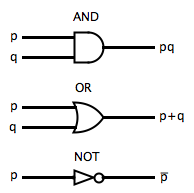
\includegraphics[width=!,height=!,scale=0.75]{AndOrNot.png}
%\begin{tikzpicture}[circuit logic US]
%\matrix[column sep=1cm]
%{
%  \node (a0) {$p$}; & \node {\textsc{and}}; & & \\
%  & \node [and gate] (a2) {}; & \node (a3) {$pq$}; & \\
%  \node (a1) {$q$}; & & & \\
%  \node (o0) {$p$}; & \node {\textsc{or}}; & & \\
%  & \node [or gate] (o2) {}; & \node (o3) {$p+q$}; & \\
%  \node (o1) {$q$}; & & & \\
%  & \node {\textsc{not}}; & \\
%  \node (n0) {$p$}; & \node [not gate] (n1) {}; & \node (n2) {$\overline{p}$}; \\
%};
%\draw (a2.input 1) -- ++(left:4mm) |- (a0.east);
%\draw (a2.input 2) -- ++(left:4mm) |- (a1.east);
%\draw (a2.output) -- (a3.west);
%\draw (o2.input 1) -- ++(left:4mm) |- (o0.east);
%\draw (o2.input 2) -- ++(left:4mm) |- (o1.east);
%\draw (o2.output) -- (o3.west);
%\draw (n1.input) -- (n0.east);
%\draw (n1.output) -- (n2.west);
%\end{tikzpicture}
\end{center}

The final result is a circuit diagram such as Figure~\ref{fig:exprcircuit}.
\begin{figure}
\begin{center}
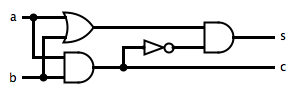
\includegraphics[width=!,height=!,scale=0.75]{HalfAdder.png}
%\begin{tikzpicture}[circuit logic US]
%\matrix[column sep=1cm]
%{
%  \node [or gate] (o1) {}; & & \node [and gate, yshift=-1mm] (a2) {}; & \node [yshift=-1mm] (s) {$s$}; \\
%  & \node [not gate] (n1) {}; & & \\
%  \node [and gate] (a1) {}; & & & \node (c) {$c$}; \\
%};
%\node (a) at ([xshift=-1.1cm]o1.input 1) {$a$};
%\node (b) at ([xshift=-1cm]a1.input 2) {$b$};
%\draw (a.east) -- (o1.input 1);
%\draw[*-] (b.east) ++(3mm,-0.8mm) |- (o1.input 2);
%\draw[*-] (a.east) ++(5mm,0.8mm) |- (a1.input 1);
%\draw (b.east) -- (a1.input 2);
%\draw (o1.output) -- ++(right:2cm) |- (a2.input 1);
%\draw (a2.output) -- (s.west);
%\draw (a1.output) -- (c.west);
%\draw[*-] (a1.output) ++(5mm,-0.8mm) |- (n1.input);
%\draw (n1.output) -- ++(right:0.5cm) |- (a2.input 2);
%\end{tikzpicture}
\end{center}
\caption{Circuit diagram for $s=(a+b)\overline{ab}$ and $c=ab$}
\label{fig:exprcircuit}
\end{figure}

It is important to realize, though, that this is just another presentation of the logical expressions we started with. Any set of Boolean expressions may be drawn this way, and any circuit where all of the information flows from left to right may be read as a set of expressions.

In addition to visualizing the layout of gates in a digital circuit, a circuit diagram may be used to ``trace'' its operation on particular inputs. For example, Figure~\ref{fig:exprcircuit11} is our example circuit annotated with \0/\1 logic values on each wire, to trace its behavior when both inputs $a$ and $b$ are 1. Since the logic values flow from left to right, the output of each successive gate may be determined from its inputs. By tracing each combination of inputs, we may construct a truth table corresponding to the circuit; the result is
\[ \begin{array}{cc|cc}
a  & b  & c & s\\ \hline
\0 & \0 & \0 & \0\\
\0 & \1 & \0 & \1\\
\1 & \0 & \0 & \1\\
\1 & \1 & \1 & \0
\end{array} \]
\begin{figure}
\begin{center}
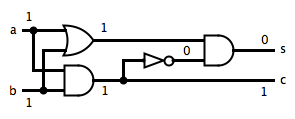
\includegraphics[width=!,height=!,scale=0.75]{HalfAdder11.png}
\end{center}
\caption{Annotated diagram for $s=(a+b)\overline{ab}$ and $c=ab$ when $a=1$ and $b=1$}
\label{fig:exprcircuit11}
\end{figure}

\paragraph{Implementation of Logic Gates}

\firstthought{It is useful} to have some idea of how digital logic gates are built out of lower-level electronic devices such as transistors. For our purposes, a transistor is a voltage-controlled switch: when the voltage is high, the switch is closed (that is, it conducts electricity); when the voltage is low, the switch is open (breaking the connection). Figure~\ref{fig:nmosgates} shows n-type metal-oxide-semiconductor (NMOS) implementations of \textsc{not}, \textsc{nor}, and \textsc{nand} gates; we will study these instead of the more common complementary MOS (CMOS) gates, because they are slightly simpler---CMOS has the practical advantage of using significantly less power, at the cost of doubling the number of transistors, but the basic principles are very similar.

\begin{figure}
\begin{center}
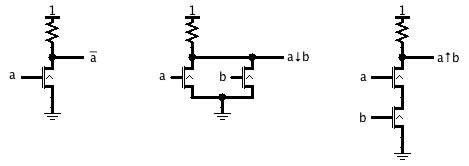
\includegraphics[width=!,height=!,scale=0.75]{NMOSgates.png}
\end{center}
\caption{NMOS implementations of \textsc{not}, \textsc{nor}, and \textsc{nand} gates}
\label{fig:nmosgates}
\end{figure}

The \textsc{not} gate consists of a single transistor in the lower half: the ``gate'' on the left is connected to the input signal, $a$; the ``source'' at the bottom is connected to ground, and the ``drain'' at the top is connected to the output, $\overline{a}$, and a ``pull-up'' resistor (the jagged line) whose other end is at the high voltage level. When $a=\0$ and the switch is open (so the transistor effectively has infinite resistance), the output will be pulled high (so $\overline{a}=\1$). When $a=\1$ and the switch is closed, the lower resistance through the transistor will pull the output low (so $\overline{a}=\0$).

The \textsc{nor} gate uses two transistors in parallel: if either $a$ or $b$ is high, then the output will be pulled low. Conversely, the \textsc{nand} gate uses two transistors in series: both have to be closed (so $a=b=\1$) for the output to be pulled to \0. Here are the conventional circuit symbols for \textsc{nand} and \textsc{nor} gates (note that the circle on the output indicates negation, just like on the \textsc{not} gate; the unnegated version of \textsc{not}, drawn as a simple triangle, is known as a ``buffer,'' because it copies its input to its output unchanged, after a short delay):
\begin{center}
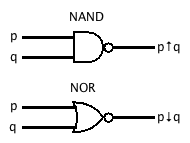
\includegraphics[width=!,height=!,scale=0.75]{NandNor.png}
\end{center}

Those three gates are the simplest to implement with transistors. As we saw in Section~\ref{ssec:OtherBooleanOps}, all other Boolean operators can be constructed from \textsc{nand} alone, or \textsc{nor} alone. For example, an \textsc{and} gate is a \textsc{nand} followed by a \textsc{not}, so it can be built out of three transistors; an \textsc{or} gate also takes three, using a \textsc{nor} and a \textsc{not}. In the next section, we will see another way to construct circuits using only \textsc{nand} gates.

\begin{tailquote}
Claude Shannon (1916--2001), known as ``the father of information theory,'' wrote his master's thesis at MIT in 1937. Entitled ``A Symbolic Analysis of Relay and Switching Circuits,'' it has been called the most influential master's thesis of the 20\textsuperscript{th} century. In it, he showed how to systematically turn expressions of Boolean algebra into circuits made up of switches.
\end{tailquote}
\begin{exercises}
\item For each of the following Boolean expressions, draw a corresponding circuit diagram. Try to reuse as many common intermediate results as you can.
\begin{enumerate}
\item $x=\overline{(\overline{a}+b)}+\overline{\overline{b}}+\overline{a}$
\item $x=\overline{\overline{c}a}+\overline{b}$, $y=\overline{\overline{c}b}+\overline{a}$
\item $x=abc+abd+acd+bcd$
\end{enumerate}

\item For each of the following truth tables, draw a corresponding circuit diagram. \textit{(Hint: First extract one or more Boolean expressions in DNF from the table.)}
\begin{enumerate}
\item \( \begin{array}[t]{cc|cc}
a  & b  & x  & y\\ \hline
\0 & \0 & \0 & \1\\
\0 & \1 & \1 & \0\\
\1 & \0 & \1 & \0\\
\1 & \1 & \0 & \1
\end{array} \)
\item \( \begin{array}[t]{ccc|c}
a  & b  & c  & x\\ \hline
\0 & \0 & \0 & \0\\
\0 & \0 & \1 & \0\\
\0 & \1 & \0 & \0\\
\0 & \1 & \1 & \1\\
\1 & \0 & \0 & \0\\
\1 & \0 & \1 & \1\\
\1 & \1 & \0 & \1\\
\1 & \1 & \1 & \1
\end{array} \)
\end{enumerate}

\item For each of the following circuit diagrams, write the corresponding Boolean expressions, then trace the output on each combination of inputs and summarize the results in a truth table.
\begin{enumerate}
\item 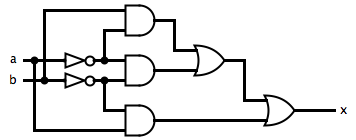
\includegraphics[width=!,height=!,scale=0.75]{Exercise5213a.png}
\item 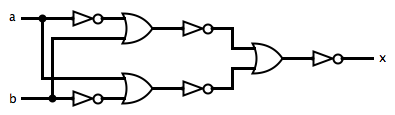
\includegraphics[width=!,height=!,scale=0.75]{Exercise5213b.png}
\end{enumerate}
\end{exercises}

\subsection{Circuit Simplification}\label{sec:circsimp}
\firstthought{As noted above,} a physical circuit does have some dependence on time, since each device in the circuit requires a non-zero time to respond to a change in its inputs. A more precise model needs to take these delays into account---a circuit is modeled by a Boolean expression \emph{plus} a set of delay factors (other cost measures may also be important: power consumption, heat production, area occupied, \textit{etc.}, but we will focus on the delay issue here). We will make the simplifying assumption that all gates have the same delay time, so we will measure the total delay of a circuit in terms of the number of gate delays required before the output values accurately reflect a change to the input values.

Given a combinational circuit, we may compute the delay, also known as the \textit{span}, by finding the number of gates on the longest path (the ``critical path'') from an input to an output. For example, the circuit in Figure~\ref{fig:exprcircuit} has a span of three gate delays, with the critical path going from either $a$ or $b$ to $s$, passing through an \textsc{and}, a \textsc{not}, and another \textsc{and} gate. Note that this is a conservative estimate of the delay required, although for certain inputs the output may become stable sooner---for example, if $a$ and $b$ both change to \0, then after one gate delay the output of the \textsc{or} and the first \textsc{and} will both be \0; that means that in this case, output $c$ will be determined after one gate delay, while output $s$ will be determined after two gate delays (because as soon as one input to the second \textsc{and} is \0, its output will become \0 after one more gate delay regardless of the other input). However, other combinations of inputs may well take the entire three gate delays to correctly determine the value of $s$.

One approach to reducing the delay of a circuit is to use the disjunctive normal form, also known as the ``sum-of-products'' (see Section~\ref{ssec:DNF}). Since an expression in DNF is the \textsc{or} of a collection of terms which are the \textsc{and} of some number of literals, and a literal is either an input or a negated input, the corresponding circuit can be constructed in three layers:
\begin{center}
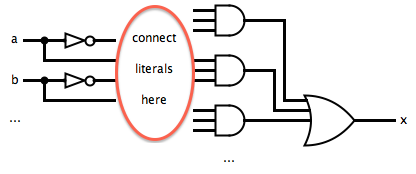
\includegraphics[width=!,height=!,scale=0.75]{DNFlayers.png}
\end{center}

An interesting property of the sum-of-products representation falls out of the De Morgan laws. Since $ab+cd=\overline{\overline{ab}\cdot\overline{cd}}=(a\uparrow b)\uparrow(c\uparrow d)$, the two layers of \textsc{and} and \textsc{or} gates may be replaced entirely with \textsc{nand} gates to get an equivalent circuit!
\begin{center}
\includegraphics[width=!,height=!,scale=0.75]{DNFlayersNand.png}
\end{center}

Unfortunately, this does not mean that any Boolean expression can be computed by a circuit with only three gate delays. One problem comes when we need \textsc{and} and \textsc{or} gates (or \textsc{nand} gates) with more than two inputs---in general, with $n$ input variables, there may be \textsc{and} gates that need $n$ literal inputs, and there could be on the order of $2^n$ gates in the \textsc{and} level, requiring an \textsc{or} gate with that many input lines. We will see in the next section how to build gates with a larger number of inputs out of gates with just two inputs.

Another problem with DNF comes if we use the full DNF expression extracted from a truth table. Recall the full DNF expression that we extracted from the truth table for $p\rightarrow q$ in Section~\ref{ssec:OtherBooleanOps}: $\overline{p}\cdot\overline{q}+\overline{p}q+pq$. We were able to use Boolean identities to find an equivalent DNF expression, $\overline{p}+q$ (which only needs two gate delays, since the \textsc{and} layer disappears). There are general techniques for finding simpler DNF expressions such as this; we will look at a simple technique called a \textit{Karnaugh map}, although for computer implementation the related Quine-McCluskey algorithm is better (and for large numbers of input variables a heuristic approach is necessary).

\newthought{A Karnaugh map} is a way of visualizing entries in a truth table so that adjacent entries only differ on the value of one input variable. For example, the entry for $\overline{p}q$ will be next to the entry for $pq$. If adjacent entries each contain 1, meaning that those terms would participate in the full DNF expression, then they may be replaced by a single term with just the variables that are the same: in the example, this corresponds to the simplification $\overline{p}q + pq=(\overline{p}+p)q=1q=q$.

For two input variables, a Karnaugh map is a $2\times 2$ array:
\[ \begin{array}{r|cc}
& \overline{q} & q\\ \hline
\overline{p} & x_{00} & x_{01}\\
p & x_{10} & x_{11}
\end{array} \]
This is just a compact rearrangement of the truth table:
\[ \begin{array}{cc|c}
p & q & x\\ \hline
\0 & \0 & x_{00}\\
\0 & \1 & x_{01}\\
\1 & \0 & x_{10}\\
\1 & \1 & x_{11}
\end{array} \]
However, note that the adjacent cell condition is true: horizontally adjacent cells only differ on $q$, while vertically adjacent cells only differ on $p$.

Once we have laid out the Karnaugh map, a simplified expression may be read off by finding a way to cover all of the 1's in the map with ``implicants.'' An implicant is a rectangle whose side lengths are a power of 2; it corresponds to finding a collection of adjacent cells in the map (all of which contain 1) that all agree on some of the input literals and that collectively include all combinations (negated or not) of the other input variables. The resulting term for an implicant is just the product of the common literals among all the cells covered by the implicant.

On a $2\times 2$ map, the only implicants are individual cells ($1\times 1$), a row ($1\times 2$), a column ($2\times 1$), or the entire map ($2\times 2$). The cells correspond to terms such as $p\overline{q}$, the rows are either $\overline{p}$ or $p$, the columns are either $\overline{q}$ or $q$, and the entire map is $1$ (the empty product). To get the simplest expression, we want to take the fewest number of the largest possible implicants that between them cover all of the 1's in the map. Implicants may overlap, as long as all of (and only) the 1's are covered by at least one implicant.

Here is the example again. First the truth table for $p\rightarrow q$:
\[ \begin{array}{cc|c}
p & q & x\\ \hline
\0 & \0 & \1\\
\0 & \1 & \1\\
\1 & \0 & \0\\
\1 & \1 & \1
\end{array} \]
As a Karnaugh map, this is:
\[ \begin{array}{r|cc}
& \overline{q} & q\\ \hline
\overline{p} & \1 & \1\\
p & \0 & \1
\end{array} \]
The best way to cover this map with implicants is to take the first row and the second column. That gives the simplified terms $\overline{p}$ and $q$, so the final simplified expression is $\overline{p} + q$. Here is the map with the implicants outlined:
\[ \begin{array}{r|cc}
& \overline{q} & q\\ \hline
\overline{p} & \tikzmark{left1}\1 & \tikzmark{left2}\1\tikzmark{right1}\\
p & \0 & \1\tikzmark{right2}
\end{array}
\DrawBox[blue]{left1}{right1}
\DrawBox[red]{left2}{right2} \]

A Karnaugh map can also work with three or four input variables, producing either a $2\times 4$ or a $4\times 4$ array. The same procedure applies, with three complications:
\begin{enumerate}
\item To satisfy the adjacent cell condition, successive rows or columns must change only one variable at a time: for example, the rows might be labelled in order $\overline{p}\cdot\overline{q}$, $\overline{p}q$, $pq$, and $p\overline{q}$;
\item Implicants may be 1, 2, or 4 rows tall by 1, 2, or 4 columns wide; and
\item Implicants may ``wrap around'' from one side of the map to the other.
\end{enumerate}
For example, on a $4\times 4$ map, one possible implicant is the middle two rows; another is the leftmost and rightmost columns (wrapping horizontally); a third is the $2\times 2$ block consisting of the middle two elements of the top row and the middle two elements of the bottom row (wrapping vertically); a final example is the last two elements of the third row. See Figure~\ref{fig:KarnaughImplicants} for these examples.

\begin{figure}
Middle two rows ($q$):
\[ \begin{array}{r|cccc}
& \overline{r}\cdot\overline{s} & \overline{r}s & rs & r\overline{s}\\ \hline
\overline{p}\cdot\overline{q} & & & & \\
\overline{p}q & \tikzmark{left1}1 & 1 & 1 & 1\\
pq & 1 & 1 & 1 & 1\tikzmark{right1}\\
p\overline{q} & & & &
\end{array}
\DrawBox[blue]{left1}{right1} \]

Leftmost and rightmost columns ($\overline{s}$):
\[ \begin{array}{r|cccc}
& \overline{r}\cdot\overline{s} & \overline{r}s & rs & r\overline{s}\\ \hline
\overline{p}\cdot\overline{q} & \tikzmark{left1}1 & & & \tikzmark{left2}1\\
\overline{p}q & 1 & & & 1\\
pq & 1 & & & 1\\
p\overline{q} & 1\tikzmark{right1} & & & 1\tikzmark{right2}
\end{array}
\DrawBoxW[blue]{left1}{right1}
\DrawBoxE[blue]{left2}{right2} \]

Middle elements of top and bottom rows ($\overline{q}s$):
\[ \begin{array}{r|cccc}
& \overline{r}\cdot\overline{s} & \overline{r}s & rs & r\overline{s}\\ \hline
\overline{p}\cdot\overline{q} & & \tikzmark{left1}1 & 1\tikzmark{right1} & \\
\overline{p}q & & & &\\
pq & & & &\\
p\overline{q} & & \tikzmark{left2}1 & 1\tikzmark{right2} &
\end{array}
\DrawBoxN[blue]{left1}{right1}
\DrawBoxS[blue]{left2}{right2} \]

Last two elements of the third row ($pqr$):
\[ \begin{array}{r|cccc}
& \overline{r}\cdot\overline{s} & \overline{r}s & rs & r\overline{s}\\ \hline
\overline{p}\cdot\overline{q} & & & & \\
\overline{p}q & & & &\\
pq & & & \tikzmark{left1}1 & 1\tikzmark{right1}\\
p\overline{q} & & & &
\end{array}
\DrawBox[blue]{left1}{right1} \]
\caption{Some examples of Karnaugh map implicants}
\label{fig:KarnaughImplicants}
\end{figure}

A Karnaugh map also allows us to find simple circuits in the case that some combinations of inputs will never occur, so that we do not care what the output is in those rows of the truth table. By entering a ``don't care'' value, such as X, in the map, we have the freedom to either ignore or include those cells when covering the map with implicants; by including a cell with an X along with a group of 1's, we might be able to construct a larger (and hence simpler) implicant.

For example, suppose we have the following truth table for a four-variable Boolean expression (this represents the inputs that are binary numbers less than ten and divisible by three):
\[ \begin{array}{cccc|c}
p & q & r & s & x\\ \hline
\0 & \0 & \0 & \0 & \1\\
\0 & \0 & \0 & \1 & \0\\
\0 & \0 & \1 & \0 & \0\\
\0 & \0 & \1 & \1 & \1\\
\0 & \1 & \0 & \0 & \0\\
\0 & \1 & \0 & \1 & \0\\
\0 & \1 & \1 & \0 & \1\\
\0 & \1 & \1 & \1 & \0\\
\1 & \0 & \0 & \0 & \0\\
\1 & \0 & \0 & \1 & \1\\
\1 & \0 & \1 & \0 & X\\
\1 & \0 & \1 & \1 & X\\
\1 & \1 & \0 & \0 & X\\
\1 & \1 & \0 & \1 & X\\
\1 & \1 & \1 & \0 & X\\
\1 & \1 & \1 & \1 & X
\end{array} \]
As a Karnaugh map, this is:
\[ \begin{array}{r|cccc}
& \overline{r}\cdot\overline{s} & \overline{r}s & rs & r\overline{s}\\ \hline
\overline{p}\cdot\overline{q} & \1 & \0 & \1 & \0\\
\overline{p}q & \0 & \0 & \0 & \1\\
pq & X & X & X & X\\
p\overline{q} & \0 & \1 & X & X
\end{array} \]
The \1's, plus some of the X's, may be covered by four implicants: $\overline{p}\cdot\overline{q}\cdot\overline{r}\cdot\overline{s}$, $\overline{q}rs$, $qr\overline{s}$, and $ps$. Note that the second implicant wraps around from the third cell on the top row to the third cell (with an X, which is also covered by the $ps$ implicant) on the bottom row; if it were just the \1 on the top row, then the term would be $\overline{p}\cdot\overline{q}rs$, which is not as simple. Here are the cells that end up being covered:
\[ \begin{array}{r|cccc}
& \overline{r}\cdot\overline{s} & \overline{r}s & rs & r\overline{s}\\ \hline
\overline{p}\cdot\overline{q} & \tikzmark{left1}\1\tikzmark{right1} & \0 & \tikzmark{left2a}\1\tikzmark{right2a} & \0\\
\overline{p}q & \0 & \0 & \0 & \tikzmark{left3}\1\\
pq & X & \tikzmark{left4}X & X & X\tikzmark{right3}\\
p\overline{q} & \0 & \1 & \tikzmark{left2b}X\tikzmark{right2b}\tikzmark{right4} & X
\end{array}
\DrawBox[blue]{left1}{right1}
\DrawBoxN[red,rounded corners=3pt]{left2a}{right2a}
\DrawBoxS[red,rounded corners=3pt]{left2b}{right2b}
\DrawBox[green]{left3}{right3}
\DrawBox[purple]{left4}{right4} \]
Therefore, the simplified expression is $\overline{p}\cdot\overline{q}\cdot\overline{r}\cdot\overline{s} + \overline{q}rs + qr\overline{s} + ps$. This may be computed by the following circuit:
\begin{center}
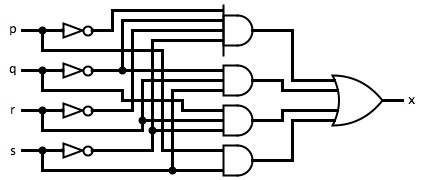
\includegraphics[width=!,height=!,scale=0.75]{KarnaughExample.png}
\end{center}
In the next section, we will see how to implement this with a total delay of 5, using only two-input \textsc{and} and \textsc{or} gates.

The final difficulty with building low-delay circuits from DNF expressions is that, even with the simplification provided by something like a Karnaugh map, many Boolean functions lead to an exponential blowup when expressed in DNF. In the worst case, an expression with $n$ input variables may require $O(2^n)$ terms in a sum-of-product representation---consider the case of a Karnaugh map where the \1's are in a checkerboard arrangement, so that none are adjacent. When $n$ is large enough, it might not even be practical to consider the truth table at all; for example, a circuit that can add two 32-bit numbers requires 64 input lines, which would lead to a truth table with $2^{64}\approx 10^{19}$ entries. The next section will also discuss approaches to this kind of problem.

\begin{tailquote}
Maurice Karnaugh [pronounced ``CAR-no''] (1924--) developed his map method in 1953, based on a 1952 paper by Edward Veitch (1924--2013), ``A Chart Method for Simplifying Truth Functions.'' The major difference between Karnaugh's and Veitch's diagrams was the ordering of the columns and rows---Veitch put them in straight binary order, while Karnaugh rearranged them to make adjacent cells differ by only one variable. Veitch's approach makes sense if you picture the diagram as showing layers of a cube or hypercube, and arguably extends more readily to five or six variables, but Karnaugh's approach became more popular.
\end{tailquote}

\begin{exercises}
\item For each of the following Boolean expressions, compute the total delay of the direct translation of the expression into a circuit.
\begin{enumerate}
\item $\overline{(\overline{p}+q)}+(\overline{\overline{q}}+\overline{p})$
\item $(\overline{\overline{r}p}+\overline{q})(\overline{\overline{r}q}+\overline{p})$
\item $(((p+q)(q+r))\,(r+s))\,(((p+r)(q+s))\,(p+s))$
\end{enumerate}

\item For each of the expressions in the previous problem, use a Karnaugh map to find an equivalent sum-of-products expression, and draw the resulting circuit.

\item Suppose we want to build a counter that cycles through the numbers 0, 1, 2, 3, 4, and back to 0. One element of this counter will be a circuit that takes the current number, expressed in binary, and outputs the next number. Here is the truth table for this function, with three inputs ($a$, $b$, and $c$) and three outputs ($x$, $y$, and $z$):
\[ \begin{array}{ccc|ccc}
a & b & c & x & y & z\\ \hline
\0 & \0 & \0 & \0 & \0 & \1\\
\0 & \0 & \1 & \0 & \1 & \0\\
\0 & \1 & \0 & \0 & \1 & \1\\
\0 & \1 & \1 & \1 & \0 & \0\\
\1 & \0 & \0 & \0 & \0 & \0\\
\1 & \0 & \1 & X & X & X\\
\1 & \1 & \0 & X & X & X\\
\1 & \1 & \1 & X & X & X\\
\end{array} \]
Since the counter should never reach numbers 5, 6, or 7, we do not care about the output when $abc$ is \1\0\1, \1\1\0, or \1\1\1. Use Karnaugh maps to find a simple circuit for this function.

\item\label{ex:BCD} In binary-coded decimal (BCD), four bits are used to represent the numbers 0 (\0\0\0\0) through 9 (\1\0\0\1); the other six bit patterns (\1\0\1\0 through \1\1\1\1) are unused. BCD is often used in circuits where decimal numbers need to be displayed; a common device for doing so is the ``seven-segment display.'' Using only seven elements (for example, light-emitting diodes), we may form a reasonable approximation of all the digits 0--9: \textifsym{0123456789}. Construct a truth table with four inputs and seven outputs showing how to produce these characters from input in BCD (be sure to include a diagram indicating which output column corresponds to which display element). Use Karnaugh maps to design a relatively simple circuit that implements a seven-segment decoder.

\item Exercise~\ref{ex:CNF} of Section~\ref{ssec:DNF} examines conjunctive normal form (CNF), the dual of DNF. Explore what kind of circuits result from CNF, and how to extract a simplified CNF expression from a Karnaugh map \textit{(Hint: look at blocks of \0's.)}.
\end{exercises}

\subsection{Common Circuit Components}
\firstthought{Just as a complicated piece of software} is never written from scratch entirely from the most basic program statements, a complicated hardware design is not approached purely at the gate level. Where a programmer will break the task into a hierarchy of objects and functions, relying on familiar idioms and existing code from program libraries to avoid reinventing the wheel, a hardware designer will use a hierarchy of functional blocks, relying on familiar patterns and existing libraries of subcircuits.

We have already seen one of these common components---the sample circuit in Figure~\ref{fig:exprcircuit} is known as the ``half adder.'' If $a$ and $b$ represent one-bit binary numbers, then $s$ is their one-bit sum and $c$ is the carry into the next bit. For example, when $a$ and $b$ are both \1, $s$ is \0 and $c$ is \1; in binary, this says $1+1=10$. We may represent this block in a circuit diagram with an appropriately named box:
\begin{center}
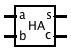
\includegraphics[width=!,height=!,scale=0.75]{HalfAdderSymbol.png}
\end{center}
It is called a half adder because, when you are adding multiple columns of bits, it only does half the work: it adds the two bits for a column, but it doesn't add in the carry from the next smaller column. A ``full adder'' takes three inputs: $a$ and $b$, plus the incoming carry, $c_\textit{\scriptsize in}$. The outputs are $s$, the sum that stays in the column, plus the outgoing carry to the next column, $c_\textit{\scriptsize out}$. We may build a full adder out of two half adders by first adding $a$ to $b$, then adding $c_\textit{\scriptsize in}$; since the highest total in a full adder is three (\1\1), we will never have a carry out of more than one of the half adders, so the resulting $c_\textit{\scriptsize out}$ is just the \textsc{or} of the two half adder carries. Here is the circuit with its block symbol and its truth table:
\[
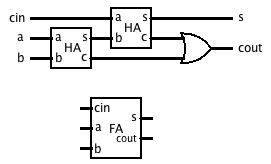
\includegraphics[width=!,height=!,scale=0.75]{FullAdder.png}\hspace{1cm}
\begin{array}[b]{ccl|rc}
a & b & c_\textit{\scriptsize in} & c_\textit{\scriptsize out} & s\\ \hline
\0 & \0 & \0 & \0 & \0\\
\0 & \0 & \1 & \0 & \1\\
\0 & \1 & \0 & \0 & \1\\
\0 & \1 & \1 & \1 & \0\\
\1 & \0 & \0 & \0 & \1\\
\1 & \0 & \1 & \1 & \0\\
\1 & \1 & \0 & \1 & \0\\
\1 & \1 & \1 & \1 & \1
\end{array}
\]

Given a full adder, we may construct multiple-bit adders by ``cascading'' them, with the carry from each column feeding into the next. Here, for example, is a four-bit adder; the inputs are $a_3a_2a_1a_0$ and $b_3b_2b_1b_0$, plus an incoming carry $c_\textit{\scriptsize in}$ to column 0 (the one's column), and the outputs are $s_3s_2s_1s_0$, plus a carry from column 3 (the eight's column), $c_\textit{\scriptsize out}$:
\begin{center}
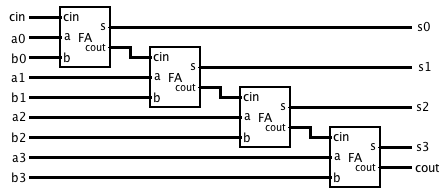
\includegraphics[width=!,height=!,scale=0.75]{4BitAdder.png}
\end{center}
Exercise~\ref{ex:cascade} explores whether this is a good design.

\newthought{A common pattern in logic circuits} is to use the \textsc{and} gate to ``enable'' (or disable) some signal. For example, in the half adder, the sum output, $s$, is true when one of the inputs is true ($a+b$), except it is disabled when there is a carry (both are true, $a\cdot b$). For another example, suppose we have a circuit which is supposed to compute one of two functions, either $f$ or $g$, depending on a ``select'' input; the circuit might look like this:
\begin{center}
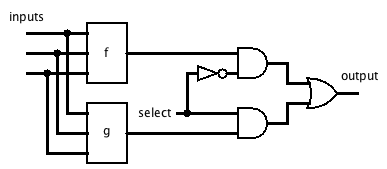
\includegraphics[width=!,height=!,scale=0.75]{ForG.png}
\end{center}
When \textit{select} is \0, the output is computed by $f$; when it is \1, the output is computed by $g$.

The idea of selecting from two signals may be generalized to using a $k$-bit input to select from one of up to $2^k$ signals; the result is known as a ``multiplexer'' (often abbreviated MUX). For example, with two select lines, $s_1s_0$, you can choose one of four inputs: $a_{00}$, $a_{01}$, $a_{10}$, or $a_{11}$. Each input is enabled by an appropriate combination of the select lines and their complements, then all four possibilities (of which at most one may be true) are combined with \textsc{or}. Here is the circuit and its common symbol:
\begin{center}
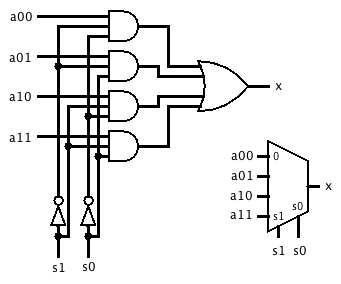
\includegraphics[width=!,height=!,scale=0.75]{MUX.png}
\end{center}

Note the similarity of the multiplexer circuit to the layers of the sum-of-products circuit from Section~\ref{sec:circsimp}. If we view the input lines $a_{ij}$ as the enabling inputs, then a multiplexer gives a direct way of implementing a truth table: hard-wire the input lines to \0 or \1 according to the corresponding entries in the truth table, then use the select lines to choose the desired row to send to the output. For example, if $a_{01}$ and $a_{10}$ are both tied to \1, while $a_{00}$ and $a_{11}$ are \0, then the output of the multiplexer will be the exclusive-\textsc{or} of $s_1$ and $s_0$.

The opposite of a multiplexer is a ``demultiplexer'' (DEMUX). It takes one input signal plus $k$ select lines, and delivers the input signal to one of $2^k$ output lines. A special case is known as a ``($k$-bit) decoder'': if the input signal is fixed at \1, then the decoder will send a \1 to exactly one of its output lines. Alternately, a demultiplexer can be viewed as a decoder with an ``enable'' input, where the selected output line will be \1 only if the enabling input signal is \1. Here is the common symbol for a four-line demultiplexer:
\begin{center}
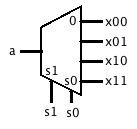
\includegraphics[width=!,height=!,scale=0.75]{DEMUX.png}
\end{center}
The implementation of this circuit is left as an exercise.

\begin{tailquote}
Edward F.~Moore (1925--2003) described his finite state machine model (see Section~\ref{sec:moore}) in a 1956 paper entitled ``Gedanken-Experiments on Sequential Machines.'' In it, he considered machines as ``black boxes,'' completely determined by their inputs and outputs (as an extreme, he considered ``infernal machines,'' where one possible output is that it explodes\ldots). The combinational circuits in this section are the special case of boxes where there is no state dependence on previous inputs.
\end{tailquote}
\begin{exercises}
\item\label{ex:cascade} Compute the total gate delays for a half adder, a full adder, and a four-bit cascaded adder as described in this section. The total delay is the maximum number of gate delays between any input signal changing and all output signals stabilizing to reflect the changed input.

\item Draw the circuit diagram for an implementation of a four-line demultiplexer.

\item A ``parity bit generator'' is a circuit that takes some number of lines of input and produces one output which is \0 if an even number of the inputs are \1, and \1 if an odd number of the inputs are \1. If the input bits are transmitted along with the generated parity bit, then a recipient can check whether any single bit was mis-transmitted by ensuring that the total number of \1 bits received is even. A two-input parity bit generator is just the exclusive-\textsc{or} circuit, whose common symbol is:
\begin{center}
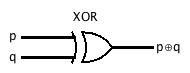
\includegraphics[width=!,height=!,scale=0.75]{XOR.png}
\end{center}
Give an implementation of a two-input parity bit generator using only \textsc{nand} gates, and then show how to use \textsc{xor} gates to build an eight-input parity bit generator.

\item The opposite of a decoder is an ``encoder'': given $2^k$ input lines, the output will be a $k$-bit binary number representing which input is \1. In case more than one input line is \1, the output will give the highest such line number; this is known as a ``priority encoder.'' For example, when $k=3$, if lines $a_1$, $a_4$, and $a_5$ are all \1, while the rest are \0, then the output will be \1\0\1 (5 in binary). If no input line is \1, then the output will be \0\0\0. There is one additional output line, $g$ (the ``group'' signal) that will only be \1 if at least one of the inputs is \1; this allows us to tell the difference between no input and only line $a_0$ being \1.

Give a truth table for a four-input ($k=2$) priority encoder, then draw a circuit diagram that implements it.
\end{exercises}

\subsection{Divide-and-Conquer Design}
\firstthought{See} Sections~13.5--7 of Aho \& Ullman.
\begin{exercises}
\item Show how to construct a $2k$-input parity bit generator given a block that implements a $k$-input parity bit generator.

\item Show how to construct a $2k$-input priority encoder given a block that implements a $k$-input priority encoder.
\end{exercises}




% !TEX root = ../root.tex

\section{Sequential Circuits}
\firstthought{All of the circuits} we have considered so far have been acyclic; this was an essential part of the definition of a combinational circuit. In general, if a circuit has a cycle, its output behavior might not be well-behaved---consider the simple example of a \textsc{not} gate whose output feeds back to its input, so that if the output went high, it would be forced low after one gate delay, then back high after another delay, \textit{etc}.\footnote{In fact, since a physical device can only be an approximation of a pure logic gate, it is more likely that the output would hover around some intermediate level, neither high nor low.}

In this section, we will explore two ways of adding cycles to circuits in a controlled fashion. The first, operating on the level of just a few gates, will give us circuit components with memory. The second, using larger-scale feedback on circuits that include both combinational and memory components, will give us a means of implementing state machines and, ultimately, general-purpose processors. On the larger scale, the circuits will be what are known as ``synchronous''---that is, a clock signal is used to synchronize the times at which feedback is applied. At the small scale, we will start with ``asynchronous'' circuits, where feedback may arrive as soon as the gate delays permit. While it is possible to design large-scale asynchronous circuits, we will not be considering that here.

Circuits with cycles are known as ``sequential logic'' circuits, because the output depends on the particular \emph{sequence} of inputs the device has received in the past; unlike combinational circuits, the output is not solely determined by the current combination of input values but potentially by the entire history of inputs (in other words, it is not purely functional---its behavior depends on side-effects). As a result, they can be considerably harder to reason about, and we will need good abstract models, such as state machines.

\subsection{Memory Devices}
\firstthought{Although the circuit} with one \textsc{not} gate feeding back on itself is unstable, a cycle of two \textsc{not} gates would be fine:
\begin{center}
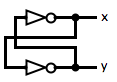
\includegraphics[width=!,height=!,scale=0.75]{NotLatch.png}
\end{center}
Whatever the output is at $x$, the output at $y$ will be the opposite. Each one feeds back and reinforces the other, and the circuit is stable. Unfortunately, it is not very useful---there is no way to provide input to \emph{change} the value $x$.

By replacing the \textsc{not} gates with either \textsc{nand} or \textsc{nor} gates, we get a circuit known as a latch. Here is the diagram for a so-called $\overline{SR}$ latch:
\begin{center}
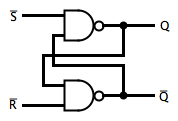
\includegraphics[width=!,height=!,scale=0.75]{SRLatch.png}
\end{center}
When the inputs $\overline{S}$ (set) and $\overline{R}$ (reset) are both \1, the latch behaves just like the circuit with two \textsc{not} gates (because $\1\uparrow x=\overline{x}$): whatever the output is at $Q$, the opposite value will be at $\overline{Q}$ (hence its customary label---it is the negation of $Q$).

When the $\overline{S}$ input is \0, the output $Q$ is forced to \1---the latch is ``set'' (the label $\overline{S}$ suggests that it is ``active-low'': the latch will be set when the input is false). Again, because of the feedback, when $Q$ is \1, $\overline{Q}$ will be \0. Returning $\overline{S}$ to \1 \emph{will then leave the latch in the set state}. This is where the sequential nature of the latch shows: its state depends on its past history (in this case, the fact that the set line was most recently active).

When the $\overline{R}$ input is \0, the output $\overline{Q}$ is forced to \1 and correspondingly $Q$ will become \0---the latch has been ``reset.'' Again, returning $\overline{R}$ to \1 will leave it in the reset state, until the set line is next activated.

If both the set and reset lines are active (\0), then both output lines will be forced to \1. This presents two problems: it violates the property that $Q$ and $\overline{Q}$ are complementary, and it sets up a potential race condition if both lines are restored to \1 at the same time. When the inputs are \1, exactly one of the outputs can be high; however, which one ``wins'' the race will depend on the precise timing of the transitions from \0 to \1, and potentially also on slight imperfections in the gates (if one of the \textsc{nand} gates responds slightly faster than the other, for example). So, don't do that.

The $\overline{SR}$ latch is what is known as a \textit{transparent} latch: the output responds as soon as the input is changed. To make sequential design easier, we frequently want memory devices that will only respond at certain times. By adding an extra layer of gates to the input, we can make what is known as a ``gated D latch.'' The inputs are $D$ (data) and $E$ (enable):
\begin{center}
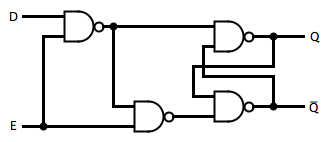
\includegraphics[width=!,height=!,scale=0.75]{DELatch.png}
\end{center}
As long as $E$ is \0 (note that this is now an active-high device), the $\overline{S}$ and $\overline{R}$ inputs to the latch will always be \1, regardless of the $D$ input. The gated D latch is only enabled when the $E$ input is \1. When enabled, the latch becomes transparent: if $D$ is \1, then $\overline{S}$ will be \0, and the output $Q$ will be set to \1; if $D$ goes to \0, then $\overline{R}$ will be \0 and the latch will be reset. There is no combination of inputs for $D$ and $E$ which can make both the set and reset lines active at the same time, so we don't have to worry about that case.

When the enable line returns to \0, the gated D latch will remain in whatever state it last entered. Here is a truth table for the latch, together with its common symbol when used in a circuit:
\[ \begin{array}[b]{cc|cc}
E & D & Q & \overline{Q}\\ \hline
\0 & X & \multicolumn{2}{c}{\textrm{last state}}\\
\1 & \0 & \0 & \1\\
\1 & \1 & \1 & \0
\end{array}\hspace{1cm}
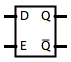
\includegraphics[width=!,height=!,scale=0.75]{DELatchSymbol.png}
\]

When dealing with a sequential circuit, it is often helpful to look at a \emph{timing diagram}, which shows the levels at various points of the circuit over time (increasing from left to right). Here is a timing diagram for the gated D latch, which shows that the output is transparent to the $D$ input only when $E$ is high:
\[ \begin{array}{cc}
E & \texttiming{2C2C2C2C}\\
D & \texttiming{LHLHLHLH}\\
Q & \texttiming{LLLHHHLH}
\end{array} \]

\newthought{Instead of a latch}, it is more common to use a device known as a ``flip-flop.'' The distinction from a latch is that a flip-flop will only respond to input for a very brief time; it is what is known as a \textit{clocked} device, since it will only change its state when a clock pulse is received (typically, just as the clock pulse is rising from \0 to \1). In \emph{synchronous} logic design, the entire circuit will use a single clock signal, so that each clock pulse advances the state by one step (and the state has time to propagate through all the gate delays before the next pulse). Here is one design for an edge-triggered D flip-flop:
\begin{center}
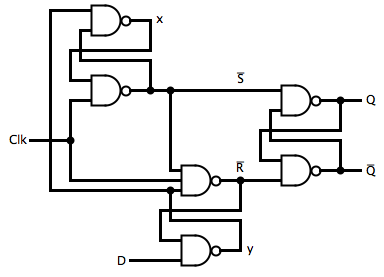
\includegraphics[width=!,height=!,scale=0.75]{DFlipFlop.png}
\end{center}
Just as the gated D latch modified an $\overline{SR}$ latch by adding a layer of two \textsc{nand} gates, this flip-flop modifies an $\overline{SR}$ latch by adding a layer of two input latches. In each case, the input layer protects the output latch from entering the illegal state (both $\overline{S}$ and $\overline{R}$ low).

The idea is that, as long as the clock (\textit{Clk}) is \0, the set ($\overline{S}$) and reset ($\overline{R}$) lines of the output latch will stay high (inactive). The line marked $x$ will be whatever $D$ is, and the line marked $y$ will be the opposite, $\overline{D}$. Although one of the input latches will be in an ``illegal'' state, the output latch will not be affected.

When the clock goes to \1, the input latches will resolve to consistent states: $\overline{S}$ will be $\overline{x}=\overline{D}$, and $\overline{R}$ will be $\overline{y}=D$. That is, if $D$ was \0, then the output latch will be reset, while if $D$ was \1 it will be set. However, once the clock reaches \1, further changes to $D$ will be ignored: if the lower input latch is reset ($\overline{R}$ is \0, meaning $D$ was \0 at the rising edge), then changing $D$ will leave it in the reset state; if instead the lower input latch is set ($\overline{R}$ is \1, meaning $D$ was \1 at the rising edge), then changing $D$ will switch it between the set and illegal states (where $\overline{R}$ is still \1), and the upper input latch will stay in the set state.

When the clock goes back to \0, the output latch will continue to hold whatever state it had (because both of its inputs will be \1 again), until the next time the clock rises.

The only danger with this design is if $D$ is changed at exactly the same time as the rising of the clock signal, because then if one of the input latches was in an illegal state it is possible to have a race condition. Designers avoid this by arranging for the $D$ input to be stable for at least a brief ``setup and hold'' time around clock pulses.

Here is a timing diagram for the D flip-flop, and its common circuit signal (the input marked with a triangle indicates that it is a rising-edge-triggered clock):
\[ \begin{array}[b]{rc}
\textit{Clk} & \texttiming{2C2C2C2C2C2C2C2C}\\
D & \texttiming{lLHLHLLLHHHLHLHHh}\\
Q & \texttiming{LLHHHHLLLLHHHHHH}
\end{array}\hspace{1cm}
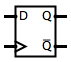
\includegraphics[width=!,height=!,scale=0.75]{DFlipFlopSymbol.png}
\]

Rather than a truth table, it is useful to give what are known as a \emph{characteristic table} or an \emph{excitation table} for a flip-flop. The characteristic table shows how the input ($D$) and current state ($Q$) lead to the next state ($Q'$) after the clock pulse:
\[ \begin{array}{cc|c}
D & Q & Q'\\ \hline
\0 & \0 & \0\\
\0 & \1 & \0\\
\1 & \0 & \1\\
\1 & \1 & \1
\end{array} \]
The excitation table presents the same information, but from the viewpoint of ``given a current state $Q$ and desired next state $Q'$, what does the input need to be?''
\[ \begin{array}{cc|c}
Q & Q' & D\\ \hline
\0 & \0 & \0\\
\0 & \1 & \1\\
\1 & \0 & \0\\
\1 & \1 & \1
\end{array} \]

\begin{tailquote}
The first electronic latch was the Eccles-Jordan trigger circuit. Patented in 1918, it was built out of two vacuum tubes connected in a feedback loop. In the early 1940's, Thomas Flowers (1905--1998) used his experience with telephone switching circuits to build Colossus, one of the code-breaking machines at Bletchley Park. The Colossus design used the Eccles-Jordan circuit as a storage register; it is considered the first programmable, electronic, digital computer, although its existence was kept secret until the 1970's.
\end{tailquote}
\begin{exercises}
\item Investigate the behavior of a latch built with \textsc{nor} gates instead of the \textsc{nand} gates used in the $\overline{SR}$ latch. Use this new latch to build a gated D latch.

\item There are several other types of flip-flops besides the D. Perhaps the most general is the JK flip-flop, which has two inputs, traditionally named $J$ and $K$, along with a clock input and the complementary $Q$ and $\overline{Q}$ outputs. When $J$ and $K$ are both \0 and a clock pulse arrives, the state does not change. When only $J$ is \1, the new state will be \1; when only $K$ is \1, the new state will be \0 (so $J$ \emph{sets} and $K$ \emph{resets} the flip-flop). Finally, when both $J$ and $K$ are \1, the clock pulse will cause the state to \emph{toggle}---that is, it will switch to the negation of its previous state. Here is the characteristic table of the JK flip-flop, using $X$ to indicate ``don't care'' inputs:
\[ \begin{array}{ccc|c}
J & K & Q & Q'\\ \hline
\0 & \0 & \0 & \0\\
\0 & \0 & \1 & \1\\
\0 & \1 & X & \0\\
\1 & \0 & X & \1\\
\1 & \1 & \0 & \1\\
\1 & \1 & \1 & \0
\end{array} \]
\begin{enumerate}
\item Draw a timing diagram that shows the behavior of the JK flip-flop.
\item Give an excitation table for the JK flip-flop.
\item Show how to construct a JK flip-flop using a D flip-flop plus a few extra gates. \textit{(Hint: Combine the $J$ and $K$ inputs with the current outputs $Q$ and $\overline{Q}$ to generate an appropriate $D$ input.)}
\end{enumerate}

\item Random-access memory (RAM) devices can be made from a quantity of flip-flops plus a few extra components such as multiplexers and demultiplexers. To store $2^k$ individually-addressable bits, you need one D type flip-flop per bit. The $D$ inputs can all be connected to an incoming data line; if each flip-flop's clock signal is driven by one line of a $k$-bit demultiplexer whose input signal is the \textsc{and} of the system clock signal and a ``write enable'' input, then the flip-flop selected by the $k$ address lines will be loaded with the desired data only if a write is enabled at the rise of the clock. Connecting the outputs of the flip-flops to a multiplexer, whose $k$ select lines are also driven by the $k$-bit address, will cause the contents of the selected bit to be passed to the output of the MUX. Use this description to draw a 16-bit RAM circuit, then show how to expand it to store four bits at each address.
\end{exercises}

\subsection{State Machines}
In Section~\ref{sec:moore} we learned about Moore machines, a version of finite state automata where there is an output associated with each state. Using flip-flops, we can build a circuit that implements a Moore machine. Here is a block diagram for such a circuit (although the connections are shown as single wires, all but the clock may be several bits wide):
\begin{center}
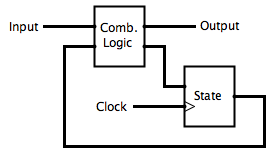
\includegraphics[width=!,height=!,scale=0.75]{MooreMachine.png}
\end{center}
In addition to the feedback within each flip-flop, there is a larger-scale feedback loop of the current state back to provide input for the next step. The box labelled ``Comb. Logic'' is a combinational circuit with two functions: compute an output based on the current state, and compute the next-state control signals based on the input and the current state. The box labelled ``State'' is one or more flip-flops; when a clock pulse arrives, it takes the control signals from the combinational logic and advances to the next state---the \emph{state} of the machine is simply the current states of these flip-flops.

If there are $k$ flip-flops, each of which can be \0 or \1, then the machine can be in $2^k$ different states. Therefore, if our Moore machine needs $n$ states, we will need at least $\lceil\lg n\rceil$ flip-flops. One step in designing the circuit for a given machine will be to assign a binary encoding to each state. For example, if the machine has three states, $A$, $B$, and $C$, then we will need two flip-flops. The circuit state will be the combination of the flip-flop outputs: $Q_1Q_0$. Given this, we may arbitrarily choose the encoding $A=\0\0$, $B=\0\1$, and $C=\1\0$ (and the state $\1\1$ will go unused).

Although the diagram shows the combinational logic has both the machine input and the current state available to compute the output, the convention in a Moore machine is that only the state is used to determine the output. There is a practical reason for this: during a clock cycle, as soon as the current state has propagated through the logic gates, we want the output to be available and stable. The input signals may not be stable until close to the end of the cycle (just before they are needed to determine the next state), and we would prefer not to see ``glitches'' in the output while the input might still be changing.

Here is an example of this process. Consider the following state machine for a mod-3 up/down counter:
\begin{center}
\begin{tikzpicture}[->,>=stealth',shorten >=1pt,auto,node distance=2.8cm,semithick]
  \node[initial,state](q0){$q_0/\0\0$};
  \node[state](q1)[right of=q0]{$q_1/\0\1$};
  \node[state](q2)[right of=q1]{$q_2/\1\0$};
  
  \path(q0) edge             node {\0} (q1)
            edge [bend left] node {\1} (q2)
       (q1) edge             node {\0} (q2)
            edge [bend left] node {\1} (q0)
       (q2) edge [bend left,in=120,out=60] node {\0} (q0)
            edge [bend left] node {\1} (q1);
\end{tikzpicture}
\end{center}
It has one input; call it $a$. When $a$ is \0, each clock pulse increments the counter through the states $q_0$, $q_1$, $q_2$, and back to $q_0$. When $a$ is \1, it decrements. At each state, the output is the corresponding number in binary: \0\0, \0\1, and \1\0.

We will use two D flip-flops, and the obvious encoding of states to bit patterns (which also happens to be the mapping from state to output, so we can just use the current state, \0\0, \0\1, or \1\0, to drive the output directly). All that remains is to design the combinational circuit that computes the $D_1$ and $D_0$ flip-flop control signals based on the input and current state. For this, we will first fill in a truth table with current state, input, and desired next state values, then use the excitation table for the flip-flops to decide an appropriate signal (for type-D flip-flops, this is particularly easy, since the required $D$ input is just the next state $Q'$):
\[ \begin{array}{ccc|cc|cc}
\multicolumn{2}{c}{\textit{current}} & \textit{input} &
  \multicolumn{2}{c}{\textit{next}} & \multicolumn{2}{c}{\textit{control}}\\
Q_1 & Q_0 & a & Q_1' & Q_0' & D_1 & D_0\\ \hline
\0 & \0 & \0 & \0 & \1 & \0 & \1\\
\0 & \0 & \1 & \1 & \0 & \1 & \0\\
\0 & \1 & \0 & \1 & \0 & \1 & \0\\
\0 & \1 & \1 & \0 & \0 & \0 & \0\\
\1 & \0 & \0 & \0 & \0 & \0 & \0\\
\1 & \0 & \1 & \0 & \1 & \0 & \1
\end{array} \]
Here is the Karnaugh map for $D_1$:
\[ \begin{array}{r|cccc}
& \overline{Q}_1\overline{Q}_0 & \overline{Q}_1Q_0 & Q_1Q_0 & Q_1\overline{Q}_0\\ \hline
\overline{a} & \0 & \tikzmark{left2}\1 & X\tikzmark{right2} & \0\\
a & \tikzmark{left1}\1\tikzmark{right1} & \0 & X & \0
\end{array}
\DrawBox[blue]{left1}{right1}
\DrawBox[red]{left2}{right2} \]
And here is the map for $D_0$:
\[ \begin{array}{r|cccc}
& \overline{Q}_1\overline{Q}_0 & \overline{Q}_1Q_0 & Q_1Q_0 & Q_1\overline{Q}_0\\ \hline
\overline{a} & \tikzmark{left1}\1\tikzmark{right1} & \0 & X & \0\\
a & \0 & \0 & \tikzmark{left2}X & \1\tikzmark{right2}
\end{array}
\DrawBox[blue]{left1}{right1}
\DrawBox[red]{left2}{right2} \]
Therefore, simple DNF expressions for the control signals are $D_1=\overline{Q}_1\overline{Q}_0a+Q_0\overline{a}$ and $D_0=\overline{Q}_1\overline{Q}_0\overline{a}+Q_1a$. The full circuit for the counter is given in Figure~\ref{fig:Mod3Counter}.
\begin{figure}
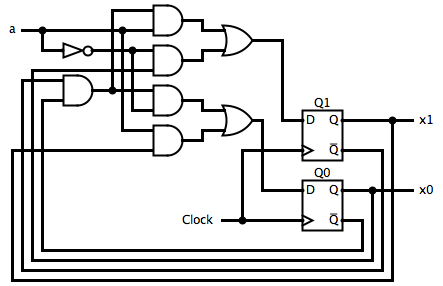
\includegraphics[width=!,height=!,scale=0.75]{Mod3Counter.png}
\caption{State machine circuit for a mod-3 up/down counter}
\label{fig:Mod3Counter}
\end{figure}

\begin{tailquote}
With combinational circuits to perform arithmetic and logic operations on data, plus registers to store intermediate results and keep track of program steps, a sequential circuit allows us to model an entire central processing unit. By connecting the inputs and outputs to external storage and I/O devices, the CPU forms the core of a general-purpose computer; details are left to the reader.
\end{tailquote}
\begin{exercises}
\item Design a BCD accumulator whose input is a three-bit two's complement number representing the value to be added to the total. That is, the state will be a decimal digit 0--9, represented in binary (\0\0\0\0 through \1\0\0\1). The output should be the signal lines to drive a seven-segment display (see Exercise~\ref{ex:BCD} of Section~\ref{sec:circsimp}). If the input is \0\0\0, then the state will be unchanged. If the input is +1 (\0\0\1) through +3 (\0\1\1), then that number will be added on each clock pulse. If the input is -4 (\1\0\0) through -1 (\1\1\1), then the total will go down by that amount on each pulse.

\item Reinterpret the block diagram for a Moore machine to produce a Mealy machine, where an output is associated with each transition. That is, the output should be determined by the current state \emph{and} the input. What might happen to the output if the input changes during a clock cycle? Compare this behavior to a Moore machine.
\end{exercises}




% !TEX root = ../root.tex

\chapter{Beyond}
Turing Machines; Halting Problem.

Also, find a place for some number theory, leading up to RSA encryption? What about combinatorics, or a bit of probability? Abstract algebra??



\backmatter

\bibliography{bibliography} % Use the bibliography.bib file for the bibliography
\bibliographystyle{plainnat} % Use the plainnat style of referencing

\cleardoublepage
\addcontentsline{toc}{chapter}{Index}
\printindex

\end{document}  
